\documentclass[11pt,a4paper]{article}
\usepackage[margin=2.5cm]{geometry}
\usepackage[T1]{fontenc}
\usepackage{lmodern}
\usepackage{microtype}
\usepackage{graphicx}
\usepackage{array}
\usepackage{booktabs}
\usepackage{longtable}
\usepackage{amsmath}
\usepackage{tikz}
\usetikzlibrary{arrows.meta, positioning}
\usepackage[font=small]{caption}
\usepackage[numbers]{natbib}
\PassOptionsToPackage{hyphens}{url}
\usepackage[hidelinks]{hyperref}
\urlstyle{tt}
\setlength{\LTcapwidth}{\textwidth}
\graphicspath{{../../output/study/part1/figures/}}

% Numbers from code: numbers.tex is generated by src/R/part1_study.R.
\makeatletter
\newcommand{\defval}[2]{\expandafter\def\csname val@#1\endcsname{#2}}
\newcommand{\val}[1]{\ifcsname val@#1\endcsname\csname val@#1\endcsname\else
  \PackageError{study}{Unknown value key `#1'}{Run Rscript src/R/part1_study.R}\fi}
\makeatother
% generated by Rscript src/R/part1_study.R; do not edit
\defval{data.n_ids}{35}  % src/R/lib/state_labels.csv
\defval{data.n_main}{30}  % in_main; src/R/lib/state_labels.csv
\defval{data.n_other_ut}{5}  % not in_main; src/R/lib/state_labels.csv
\defval{data.n_variants}{46}  % rows; src/py/btpdata/state_crosswalk.csv
\defval{data.n_quarters}{34}  % load_part1(); data/interim/phonepe.csv
\defval{data.n_phonepe_names}{36}  % raw names; data/raw/phonepe/repo/data/map/transaction/hover/country/india/2026/2.json
\defval{data.rows.phonepe}{3{,}570}  % rows; data/interim/phonepe.csv
\defval{data.rows.types}{3{,}570}  % rows; data/interim/phonepe_types.csv
\defval{data.rows.population}{1{,}190}  % rows; data/interim/population.csv
\defval{check.type_sum.n}{1{,}224}  % type_sum_equals_state_total n_items; data/interim/phonepe_checks.csv
\defval{check.type_sum.flagged}{0}  % type_sum_equals_state_total n_flagged; data/interim/phonepe_checks.csv
\defval{check.zero_fill.n}{3{,}672}  % absent_type_set_to_zero n_items; data/interim/phonepe_checks.csv
\defval{check.zero_fill.flagged}{1}  % absent_type_set_to_zero n_flagged; data/interim/phonepe_checks.csv
\defval{check.nat_count.n}{34}  % national_count_equals_state_sum n_items; data/interim/phonepe_checks.csv
\defval{check.nat_count.flagged}{0}  % national_count_equals_state_sum n_flagged; data/interim/phonepe_checks.csv
\defval{check.nat_users.n}{34}  % national_users_equals_state_sum n_items; data/interim/phonepe_checks.csv
\defval{check.nat_users.flagged}{0}  % national_users_equals_state_sum n_flagged; data/interim/phonepe_checks.csv
\defval{check.users_fall.n}{1{,}155}  % consecutive-quarter pairs, diff(users), load_part1(); data/interim/phonepe.csv
\defval{check.users_fall.flagged}{0}  % pairs with a fall in users, diff(users), load_part1(); data/interim/phonepe.csv
\defval{pop.ncp_n_rows}{37}  % state rows per year, ncp_n_rows(); data/manual/population_ncp2020.csv
\defval{pop.ncp_ratio.2018}{1.0000015}  % state rows / india row; data/manual/population_ncp2020.csv
\defval{pop.ncp_diff.2018}{2}  % state rows - india row, thousand persons, ncp_diff(); data/manual/population_ncp2020.csv
\defval{pop.ncp_ratio.2027}{0.9999993}  % state rows / india row; data/manual/population_ncp2020.csv
\defval{pop.ncp_diff.2027}{$-$1}  % state rows - india row, thousand persons, ncp_diff(); data/manual/population_ncp2020.csv
\defval{pop.total.2018Q1}{1{,}318.7}  % sum of population; data/interim/population.csv
\defval{pop.total.2026Q2}{1{,}426.0}  % sum of population; data/interim/population.csv
\defval{pop.growth_pct}{8.1}  % percent change 2018Q1-2026Q2; data/interim/population.csv
\defval{pop.growth.max.name}{Dadra and Nagar Haveli and Daman and Diu}  % 35 ids; data/interim/population.csv
\defval{pop.growth.max}{75.5}  % percent change 2018Q1-2026Q2, 35 ids; data/interim/population.csv
\defval{pop.growth.min.name}{Odisha}  % 35 ids; data/interim/population.csv
\defval{pop.growth.min}{2.8}  % percent change 2018Q1-2026Q2, 35 ids; data/interim/population.csv
\defval{pop.growth.main.max.name}{Delhi}  % main sample; data/interim/population.csv
\defval{pop.growth.main.max}{16.5}  % percent change 2018Q1-2026Q2, main sample; data/interim/population.csv
\defval{nat.count.2018Q1}{0.14}  % national(); data/interim/phonepe.csv
\defval{nat.amount.2018Q1}{0.17}  % national(); data/interim/phonepe.csv
\defval{nat.users.2018Q1}{47.5}  % national(); data/interim/phonepe.csv
\defval{nat.count.2018Q4}{0.43}  % national(); data/interim/phonepe.csv
\defval{nat.amount.2018Q4}{0.67}  % national(); data/interim/phonepe.csv
\defval{nat.users.2018Q4}{103.0}  % national(); data/interim/phonepe.csv
\defval{nat.count.2026Q2}{38.66}  % national(); data/interim/phonepe.csv
\defval{nat.amount.2026Q2}{45.50}  % national(); data/interim/phonepe.csv
\defval{nat.users.2026Q2}{711.7}  % national(); data/interim/phonepe.csv
\defval{nat.count_ratio}{276}  % 2026Q2 / 2018Q1, national(); data/interim/phonepe.csv
\defval{nat.count_rate}{82.3}  % annual_rate() 2018Q4-2026Q2, national(); data/interim/phonepe.csv
\defval{nat.amount_ratio}{264}  % 2026Q2 / 2018Q1, national(); data/interim/phonepe.csv
\defval{nat.amount_rate}{75.4}  % annual_rate() 2018Q4-2026Q2, national(); data/interim/phonepe.csv
\defval{nat.users_ratio}{15}  % 2026Q2 / 2018Q1, national(); data/interim/phonepe.csv
\defval{nat.users_rate}{29.4}  % annual_rate() 2018Q4-2026Q2, national(); data/interim/phonepe.csv
\defval{nat.count_pc.2018Q1}{0.11}  % national(); data/interim/{phonepe,population}.csv
\defval{nat.users_per_1000.2018Q1}{36}  % national(); data/interim/{phonepe,population}.csv
\defval{nat.count_pc.2018Q4}{0.32}  % national(); data/interim/{phonepe,population}.csv
\defval{nat.users_per_1000.2018Q4}{78}  % national(); data/interim/{phonepe,population}.csv
\defval{nat.count_pc.2026Q2}{27.11}  % national(); data/interim/{phonepe,population}.csv
\defval{nat.users_per_1000.2026Q2}{499}  % national(); data/interim/{phonepe,population}.csv
\defval{nat.qoq.count.2020Q2}{$-$10.6}  % qoq_count, national(); data/interim/phonepe.csv
\defval{nat.qoq.amount.2020Q2}{$-$1.9}  % qoq_amount, national(); data/interim/phonepe.csv
\defval{nat.n_qoq_neg_count}{1}  % quarters with qoq_count < 0, national(); data/interim/phonepe.csv
\defval{nat.qoq.count.median_last8}{5.9}  % median qoq_count 2024Q3-2026Q2, national(); data/interim/phonepe.csv
\defval{nat.n_states_fall.2020Q2}{16}  % ids with count 2020Q2 < 2020Q1, load_part1(); data/interim/phonepe.csv
\defval{nat.atv.2018Q1}{1{,}232}  % atv, national(); data/interim/phonepe.csv
\defval{nat.atv.peak}{1{,}907}  % max atv, national(); data/interim/phonepe.csv
\defval{nat.atv.peak_period}{2020Q3}  % period of max atv, national(); data/interim/phonepe.csv
\defval{nat.atv.2026Q2}{1{,}177}  % atv, national(); data/interim/phonepe.csv
\defval{nat.share.p2p.2018Q1}{33.6}  % national(); data/interim/{phonepe,phonepe_types}.csv
\defval{nat.share.retail.2018Q1}{64.2}  % national(); data/interim/{phonepe,phonepe_types}.csv
\defval{nat.share.utility.2018Q1}{2.1}  % national(); data/interim/{phonepe,phonepe_types}.csv
\defval{nat.share.p2p.2018Q4}{46.7}  % national(); data/interim/{phonepe,phonepe_types}.csv
\defval{nat.share.retail.2018Q4}{49.5}  % national(); data/interim/{phonepe,phonepe_types}.csv
\defval{nat.share.utility.2018Q4}{3.7}  % national(); data/interim/{phonepe,phonepe_types}.csv
\defval{nat.share.p2p.2026Q2}{30.8}  % national(); data/interim/{phonepe,phonepe_types}.csv
\defval{nat.share.retail.2026Q2}{63.9}  % national(); data/interim/{phonepe,phonepe_types}.csv
\defval{nat.share.utility.2026Q2}{5.4}  % national(); data/interim/{phonepe,phonepe_types}.csv
\defval{nat.share.retail.min2018}{38.4}  % min share_retail 2018Q1-2018Q4, national(); data/interim/{phonepe,phonepe_types}.csv
\defval{nat.share.retail.max2018}{64.2}  % max share_retail 2018Q1-2018Q4, national(); data/interim/{phonepe,phonepe_types}.csv
\defval{st.count_pc.max.name.2018Q4}{Delhi}  % main sample, load_part1(); data/interim/{phonepe,phonepe_types,population}.csv
\defval{st.count_pc.max.2018Q4}{1.26}  % main sample, load_part1(); data/interim/{phonepe,phonepe_types,population}.csv
\defval{st.count_pc.min.name.2018Q4}{Mizoram}  % main sample, load_part1(); data/interim/{phonepe,phonepe_types,population}.csv
\defval{st.count_pc.min.2018Q4}{0.06}  % main sample, load_part1(); data/interim/{phonepe,phonepe_types,population}.csv
\defval{st.count_pc.maxmin.2018Q4}{22.6}  % max/min, main sample, load_part1(); data/interim/{phonepe,phonepe_types,population}.csv
\defval{st.count_pc.max.name.2026Q2}{Telangana}  % main sample, load_part1(); data/interim/{phonepe,phonepe_types,population}.csv
\defval{st.count_pc.max.2026Q2}{100.30}  % main sample, load_part1(); data/interim/{phonepe,phonepe_types,population}.csv
\defval{st.count_pc.min.name.2026Q2}{Manipur}  % main sample, load_part1(); data/interim/{phonepe,phonepe_types,population}.csv
\defval{st.count_pc.min.2026Q2}{3.15}  % main sample, load_part1(); data/interim/{phonepe,phonepe_types,population}.csv
\defval{st.count_pc.maxmin.2026Q2}{31.8}  % max/min, main sample, load_part1(); data/interim/{phonepe,phonepe_types,population}.csv
\defval{st.users_per_1000.max.name}{Telangana}  % 2026Q2, main sample, load_part1(); data/interim/{phonepe,phonepe_types,population}.csv
\defval{st.users_per_1000.max}{943}  % 2026Q2, main sample, load_part1(); data/interim/{phonepe,phonepe_types,population}.csv
\defval{st.users_per_1000.min.name}{Meghalaya}  % 2026Q2, main sample, load_part1(); data/interim/{phonepe,phonepe_types,population}.csv
\defval{st.users_per_1000.min}{238}  % 2026Q2, main sample, load_part1(); data/interim/{phonepe,phonepe_types,population}.csv
\defval{st.intensity.max.name}{Telangana}  % 2026Q2, main sample, load_part1(); data/interim/{phonepe,phonepe_types,population}.csv
\defval{st.intensity.max}{106.3}  % 2026Q2, main sample, load_part1(); data/interim/{phonepe,phonepe_types,population}.csv
\defval{st.intensity.min.name}{Manipur}  % 2026Q2, main sample, load_part1(); data/interim/{phonepe,phonepe_types,population}.csv
\defval{st.intensity.min}{12.2}  % 2026Q2, main sample, load_part1(); data/interim/{phonepe,phonepe_types,population}.csv
\defval{st.rank_cor}{0.892}  % spearman() count_pc 2018Q4 vs 2026Q2, main sample, load_part1(); data/interim/{phonepe,phonepe_types,population}.csv
\defval{st.reach_intensity_cor}{0.600}  % spearman() users_per_1000 vs intensity 2026Q2, main sample, load_part1(); data/interim/{phonepe,phonepe_types,population}.csv
\defval{conc.top5.names.2018Q4}{Maharashtra, Karnataka, Uttar Pradesh, Andhra Pradesh and West Bengal}  % top_k(), 35 ids, load_part1(); data/interim/{phonepe,phonepe_types,population}.csv
\defval{conc.top5.count.2018Q4}{46.2}  % top_k(), 35 ids, load_part1(); data/interim/{phonepe,phonepe_types,population}.csv
\defval{conc.top5.population.2018Q4}{42.2}  % top_k(), 35 ids, load_part1(); data/interim/{phonepe,phonepe_types,population}.csv
\defval{conc.n_half.2018Q4}{6}  % n_for_share(count, 0.5), 35 ids, load_part1(); data/interim/{phonepe,phonepe_types,population}.csv
\defval{conc.top5.names.2026Q2}{Maharashtra, Karnataka, Telangana, Uttar Pradesh and Andhra Pradesh}  % top_k(), 35 ids, load_part1(); data/interim/{phonepe,phonepe_types,population}.csv
\defval{conc.top5.count.2026Q2}{52.6}  % top_k(), 35 ids, load_part1(); data/interim/{phonepe,phonepe_types,population}.csv
\defval{conc.top5.population.2026Q2}{37.5}  % top_k(), 35 ids, load_part1(); data/interim/{phonepe,phonepe_types,population}.csv
\defval{conc.n_half.2026Q2}{5}  % n_for_share(count, 0.5), 35 ids, load_part1(); data/interim/{phonepe,phonepe_types,population}.csv
\defval{dec.2018Q4.var_y}{0.595}  % decompose(), main sample, load_part1(); data/interim/{phonepe,phonepe_types,population}.csv
\defval{dec.2018Q4.var_r}{0.397}  % decompose(), main sample, load_part1(); data/interim/{phonepe,phonepe_types,population}.csv
\defval{dec.2018Q4.var_i}{0.069}  % decompose(), main sample, load_part1(); data/interim/{phonepe,phonepe_types,population}.csv
\defval{dec.2018Q4.reach}{0.776}  % decompose(), main sample, load_part1(); data/interim/{phonepe,phonepe_types,population}.csv
\defval{dec.2018Q4.intensity}{0.224}  % decompose(), main sample, load_part1(); data/interim/{phonepe,phonepe_types,population}.csv
\defval{dec.2026Q2.var_y}{0.723}  % decompose(), main sample, load_part1(); data/interim/{phonepe,phonepe_types,population}.csv
\defval{dec.2026Q2.var_r}{0.140}  % decompose(), main sample, load_part1(); data/interim/{phonepe,phonepe_types,population}.csv
\defval{dec.2026Q2.var_i}{0.305}  % decompose(), main sample, load_part1(); data/interim/{phonepe,phonepe_types,population}.csv
\defval{dec.2026Q2.reach}{0.386}  % decompose(), main sample, load_part1(); data/interim/{phonepe,phonepe_types,population}.csv
\defval{dec.2026Q2.intensity}{0.614}  % decompose(), main sample, load_part1(); data/interim/{phonepe,phonepe_types,population}.csv
\defval{dec.var_y.max}{1.255}  % max over quarters, decompose(), main sample, load_part1(); data/interim/{phonepe,phonepe_types,population}.csv
\defval{dec.var_y.max_period}{2019Q4}  % period of max var_y, decompose(), main sample, load_part1(); data/interim/{phonepe,phonepe_types,population}.csv
\defval{retail.cor.2026Q2}{0.625}  % spearman() share_retail vs count_pc 2026Q2, main sample, load_part1(); data/interim/{phonepe,phonepe_types,population}.csv
\defval{retail.max.name}{Delhi}  % 2026Q2, main sample, load_part1(); data/interim/{phonepe,phonepe_types,population}.csv
\defval{retail.max}{68.5}  % share_retail 2026Q2, main sample, load_part1(); data/interim/{phonepe,phonepe_types,population}.csv
\defval{retail.min.name}{Manipur}  % 2026Q2, main sample, load_part1(); data/interim/{phonepe,phonepe_types,population}.csv
\defval{retail.min}{43.5}  % share_retail 2026Q2, main sample, load_part1(); data/interim/{phonepe,phonepe_types,population}.csv


\title{Digital payment adoption across Indian states, 2018--2026:\\
  building the state panel from PhonePe Pulse\\[0.5ex]
  \large BTP study, Part 1}
\author{Devansh Gupta}
\date{November 2026}

\begin{document}
\maketitle

\begin{abstract}
This study builds a state-quarter panel of digital payment adoption in India. NPCI publishes UPI data by state only from April 2025. Thus the panel uses PhonePe Pulse, the open data of a UPI payment app, at one fixed commit. The panel has \val{data.n_ids} state units and \val{data.n_quarters} quarters, from 2018Q1 to 2026Q2. It gives the transaction count, the amount, the registered users and the count by type. The denominator is the quarterly population from a linear interpolation of the NCP 2020 projections. All checks between the files of the source pass, and all values are nominal. The national count increases from \val{nat.count.2018Q4} billion transactions in 2018Q4 to \val{nat.count.2026Q2} billion in 2026Q2, an annual rate of \val{nat.count_rate} percent. The average transaction value rises to Rs.~\val{nat.atv.peak} in \val{nat.atv.peak_period} and falls to Rs.~\val{nat.atv.2026Q2} in 2026Q2. In the same years, the retail share of the count increases to \val{nat.share.retail.2026Q2} percent. Across the \val{data.n_main} states of the main sample, the count per person in 2026Q2 goes from \val{st.count_pc.min.2026Q2} to \val{st.count_pc.max.2026Q2} transactions per quarter. The Spearman rank correlation of the state values in 2018Q4 and 2026Q2 is \val{st.rank_cor}. A variance decomposition divides the differences between states into reach and intensity. Reach gives the larger contribution in 2018Q4 (\val{dec.2018Q4.reach}), and intensity gives the larger contribution in 2026Q2 (\val{dec.2026Q2.intensity}).
\end{abstract}

\section{Introduction}\label{sec:intro}

\subsection{The question and the data gap}
This study is Part 1 of a B.Tech project on digital payments and financial inclusion across the states of India. The project asks whether the states that adopted digital payments faster also became more financially inclusive and grew faster. It also asks in which direction the relation goes. Adoption can increase inclusion, inclusion can make adoption faster, or both can occur. The measure of adoption is the use of the Unified Payments Interface (UPI). UPI is the real-time payment system that the National Payments Corporation of India (NPCI) operates.

These questions need data on adoption for each state over many periods. Data for one period show which states have more adoption. They cannot show whether a change in adoption comes before or after a change in inclusion. The methods of the project use the changes within each state over time: fixed-effects panel regressions and tests of the direction of the relation. These methods need a state panel, that is, one value for each state in each period. The states also differ in population, so the panel must divide each total by the population of the state.

NPCI publishes UPI statistics, but its data by state start only in April 2025 \citep{npci_upi_state, medianama2025npci}. A panel from the NPCI data thus has no quarter before April 2025. It cannot show how adoption changed in the years before 2025. The project therefore needs another source with data by state over a longer period.

\subsection{PhonePe Pulse as a proxy}
PhonePe is a digital payment app that uses UPI. The company publishes PhonePe Pulse, an open data repository with transaction counts and amounts, and user counts, for each state and each quarter from 2018Q1 \citep{phonepe_pulse}. This study uses PhonePe Pulse as the measure of adoption. The data cover the payments of one app, not all UPI payments. Part 2 of the project compares the PhonePe values with the NPCI state data for the quarters that both sources cover.

\citet{reddy2024icrier} used the state and district data of PhonePe Pulse to study how UPI spread across India. They found that the regions with high early adoption stayed ahead, with little change in the ranks of states and districts. Their paper uses an earlier release of the data. The release that this study uses restates all quarters with new definitions (Section~\ref{sec:pulse}). Thus their numbers and the numbers in this study are not comparable.

\subsection{Aim and contents of this part}
The aim of this part is to build the state-quarter panel of PhonePe adoption and its population denominator, to check it, and to describe it. The panel has \val{data.n_ids} state units and \val{data.n_quarters} quarters, from 2018Q1 to 2026Q2. Statistics across states use a main sample of \val{data.n_main} units. All values in this part are nominal: the study does not adjust the amounts for changes in prices.

Section~\ref{sec:data} describes the data sources and the files that the study uses. Section~\ref{sec:construction} explains how the raw files become the panel: the state units, the parsing rules, the data checks, the quarterly population and the measures. Section~\ref{sec:national} describes adoption in India as a whole. Section~\ref{sec:states} compares the states. Section~\ref{sec:limits} gives the limitations of the data, and Section~\ref{sec:conclusions} gives the conclusions. Appendix~\ref{app:units} lists the state units, and Appendix~\ref{app:repro} gives the commands that make all the numbers again. Part 2 of the project converts the amounts to real values with consumer price indices. It also compares PhonePe Pulse with the NPCI state data and shows the data on maps. Part 3 tests whether the states with low adoption move closer to the leading states over time (convergence).

\section{Data sources}\label{sec:data}
The panel has data from PhonePe Pulse for adoption and from the population projections of the National Commission on Population (NCP 2020) for the denominator. This section describes each source and the files that the study uses.

\subsection{PhonePe Pulse}\label{sec:pulse}
PhonePe Pulse is a public Git repository on GitHub. In it, PhonePe publishes aggregate and anonymised counts of the transactions and users of its app \citep{phonepe_pulse}. The licence is the Community Data License Agreement -- Permissive, Version 2.0 (CDLA-Permissive-2.0). This licence lets any person use, change and share the data, if the licence text goes with the shared data. PhonePe adds new data to the repository each quarter. Thus the study uses the data at one fixed commit: \texttt{257bf38}, of 24 September 2026. All PhonePe values in this study come from this commit.

The \texttt{data} folder of the commit has the sections \texttt{aggregated}, \texttt{map} and \texttt{top}. Each section has folders for transactions, users and merchants. The \texttt{aggregated} files give totals for India and for each state, with the transactions split by type. The \texttt{map} files give values by state (the ``hover'' files) and by district. The \texttt{top} files list the states and districts with the largest values. Each JSON file holds one quarter. For example, the file \texttt{2021/1.json} has the data for January to March 2021.

The commit is a new release of the data. Its README says that PhonePe restated the earlier quarters, from January--March 2018, with new definitions of the metrics. The README also advises users not to compare figures from this release with figures that PhonePe published before. It advises users not to join the data of this release and of earlier releases into one series. This study follows that rule: it uses only the files of the pinned commit.

Table~\ref{tab:files} lists the files that the study uses, with their content and the number of items.

\begin{table}[tbp]
\centering
\caption{PhonePe Pulse files used in the study. Unit: state-quarter. Sample: \val{data.n_phonepe_names} raw state and union-territory names, \val{data.n_quarters} quarters, 2018Q1--2026Q2. Source: \citet{phonepe_pulse}, pinned commit.}\label{tab:files}
\small
\begin{tabular}{@{}>{\raggedright\arraybackslash}p{4.6cm} >{\raggedright\arraybackslash}p{5.6cm} >{\raggedright\arraybackslash}p{4.6cm}@{}}
\toprule
Folder (under \texttt{data/}) & Content and use & Items \\
\midrule
\path{map/transaction/hover} & Transaction count and amount by state & \val{data.n_quarters} quarter files; \val{data.rows.phonepe} rows in the interim file \\
\path{map/user/hover} & Registered users by state & \val{data.n_quarters} quarter files; in the same interim file \\
\path{aggregated/transaction/country/india/state} & Transaction count by type: P2P, Retail, Utility & \val{data.n_phonepe_names} names $\times$ \val{data.n_quarters} quarters; \val{data.rows.types} rows in the interim file \\
\path{aggregated/transaction/country} and \texttt{aggregated/user/country} & National totals, used for checks only & \val{data.n_quarters} quarter files each \\
\bottomrule
\end{tabular}
\end{table}

The transaction hover file of a quarter has one entry for each state and union territory. Each entry gives the number of transactions in the quarter (the count) and their total value (the amount). The README does not state the unit of the amount. This study reads it as nominal rupees. The user hover file gives the number of registered users of each state in the quarter. The README does not say whether this number is cumulative. The number never falls from one quarter to the next in any state (Section~\ref{sec:checks}). This result agrees with a cumulative count of registrations. Each hover file has \val{data.n_phonepe_names} raw names. The interim file \path{phonepe.csv} has \val{data.rows.phonepe} rows: one row for each state id, quarter and variable.

The aggregated state files split the count of each state by type. The README defines the types as follows. P2P transactions are person-to-person money transfers. Utility transactions are recharges and bill payments. Business transactions are payments to merchants. This type replaces the earlier types for financial services, merchants and others. The files use the label ``Retail'' for the business type, and this study uses the file labels. The README says that the types do not overlap and that they sum to the total count. The type files give counts only, with no amounts. Thus the study can split the count by type, but not the amount. The interim file \path{phonepe_types.csv} has \val{data.rows.types} rows: one row for each state id, quarter and type. The national files of the \texttt{aggregated} section give the total count and users of India. The study uses them only to check the state files (Section~\ref{sec:checks}).

\subsection{Files not used}
The study does not use the merchant files. The README defines registered merchants as the life-till-date count of unique merchants on the platform. In each quarter from 2018Q1 to 2019Q2, one or more raw units have no merchant file. A panel of merchants would need values for these gaps, and the data do not give them.

The study does not use the district files or the top lists. The unit of the project is the state. District data would need a separate crosswalk of district names, and this study does not make one. The top lists give only the units with the largest values in a quarter, so they do not cover all units.

The pinned commit has no files on insurance, on app opens or on the device brands of users. The README still describes the user data as ``broken down by devices''. But the user files at this commit give only the registered count.

\subsection{NCP 2020 population projections}
The denominator is the projected population from the report of the Technical Group on Population Projections. The National Commission on Population issued this report, and the cover of the report gives the date November 2019 \citep{ncp2020}. The report projects the population of India and of each state and union territory for each year from 2011 to 2036. For the states except Goa, and for Delhi and the union territory of Jammu and Kashmir, the report uses the component method. This method projects fertility, mortality and migration from the 2011 Census and the Sample Registration System. The report applies it to the north-eastern states other than Assam as one group. For Ladakh, the report uses the difference between its projections for the former state and the union territory of Jammu and Kashmir. For Goa and the other union territories, it uses a mathematical method. This method fits exponential growth rates by least squares to the Census growth rates from 1981 to 2011.

The study uses Table 8 of the report. This table gives the projected total population, in thousands of persons, on 1 March of each year. The study uses the years 2018 to 2027. In each year, the table has \val{pop.ncp_n_rows} rows for the states and union territories and a row for India. A Python module reads the table from the PDF of the report into the file \path{data/manual/population_ncp2020.csv}. Section~\ref{sec:population} explains how the annual values become quarterly values, and why the panel needs the year 2027.

\subsection{Data flow}
Figure~\ref{fig:flow} shows the path of the data from the raw files to the outputs of the study. The top row has the raw sources. The second row has the Python modules that read them. Each module writes interim files in a long format, with one row for each state id, period and variable. The module \texttt{parse\_phonepe\_types} also writes the file of data checks. The R script \texttt{part1\_study.R} reads the interim files. It writes all the figures, the tables and the numbers of this study. The text gets each number from the file \path{numbers.tex} that the script writes, so the text has no hand-typed data value (Appendix~\ref{app:repro}).


\begin{figure}[htbp]
\centering
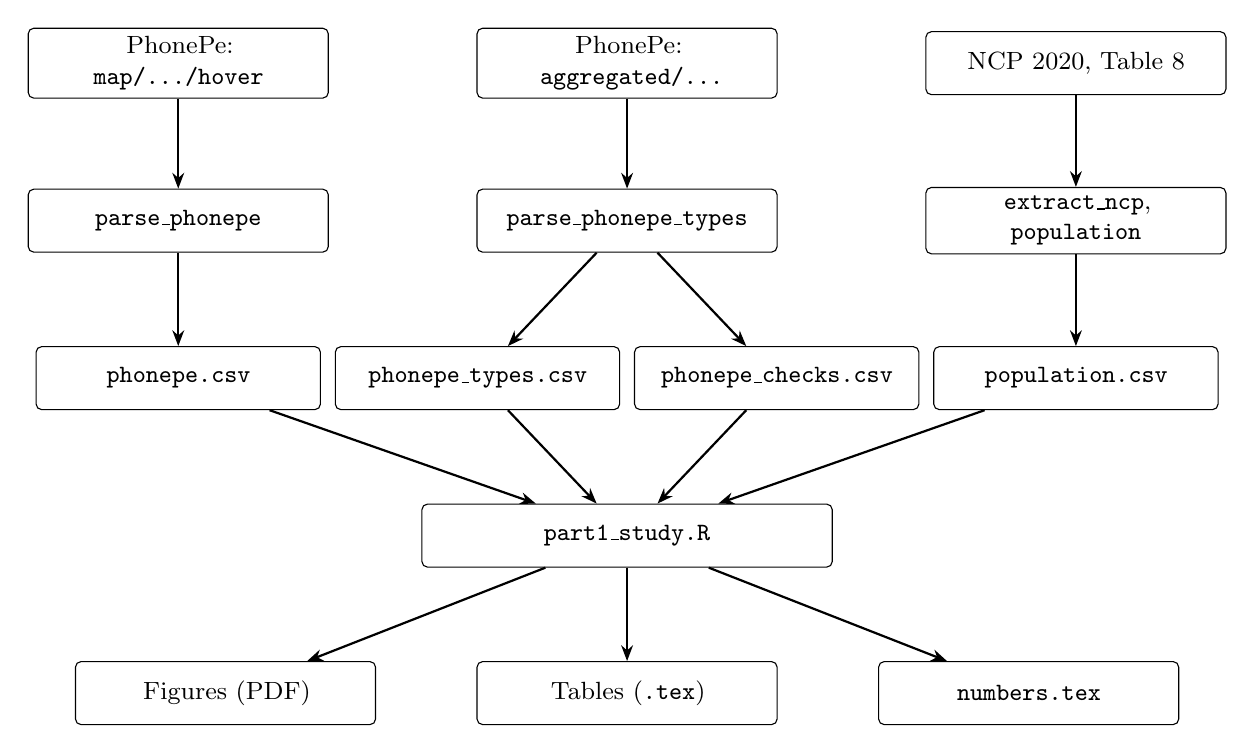
\begin{tikzpicture}[
  font=\small,
  box/.style={draw, rounded corners=2pt, align=center, minimum height=8mm, inner sep=3pt, text width=3.6cm},
  wide/.style={box, text width=5cm},
  arr/.style={-{Stealth[length=2mm]}, thick},
  node distance=6mm and 6mm]
  \node[box] (hover) at (1.8,0) {PhonePe: \texttt{map/\ldots/hover}};
  \node[box] (agg) at (7.5,0) {PhonePe: \texttt{aggregated/\ldots}};
  \node[box] (ncp) at (13.2,0) {NCP 2020, Table 8};
  \node[box] (m1) at (1.8,-2) {\texttt{parse\_phonepe}};
  \node[box] (m2) at (7.5,-2) {\texttt{parse\_phonepe\_types}};
  \node[box] (m3) at (13.2,-2) {\texttt{extract\_ncp}, \texttt{population}};
  \node[box, text width=3.4cm] (i1) at (1.8,-4) {\texttt{phonepe.csv}};
  \node[box, text width=3.4cm] (i2) at (5.6,-4) {\texttt{phonepe\_types.csv}};
  \node[box, text width=3.4cm] (i3) at (9.4,-4) {\texttt{phonepe\_checks.csv}};
  \node[box, text width=3.4cm] (i4) at (13.2,-4) {\texttt{population.csv}};
  \node[wide] (r) at (7.5,-6) {\texttt{part1\_study.R}};
  \node[box] (o1) at (2.4,-8) {Figures (PDF)};
  \node[box] (o2) at (7.5,-8) {Tables (\texttt{.tex})};
  \node[box] (o3) at (12.6,-8) {\texttt{numbers.tex}};
  \draw[arr] (hover) -- (m1);
  \draw[arr] (agg) -- (m2);
  \draw[arr] (ncp) -- (m3);
  \draw[arr] (m1) -- (i1);
  \draw[arr] (m2) -- (i2);
  \draw[arr] (m2) -- (i3);
  \draw[arr] (m3) -- (i4);
  \draw[arr] (i1) -- (r);
  \draw[arr] (i2) -- (r);
  \draw[arr] (i3) -- (r);
  \draw[arr] (i4) -- (r);
  \draw[arr] (r) -- (o1);
  \draw[arr] (r) -- (o2);
  \draw[arr] (r) -- (o3);
\end{tikzpicture}
\caption{Data flow from the raw sources to the study outputs. Raw files: \citet{phonepe_pulse} and \citet{ncp2020}. Top row: raw sources; second row: Python modules; third row: interim files; then the R script and its outputs. All interim files except the check file have the columns \texttt{state\_id}, \texttt{period}, \texttt{variable}, \texttt{value} and \texttt{source}.}\label{fig:flow}
\end{figure}

\section{Construction of the panel}\label{sec:construction}
This section explains how the raw files become the panel. It describes the state units, the parsing rules, the data checks, the quarterly population and the measures.

\subsection{State units and the crosswalk}\label{sec:units}
The sources do not use the same names for the states. For example, NCP 2020 writes ``NCT of Delhi'' and PhonePe Pulse writes ``delhi''. A crosswalk file gives the state id for each name variant. Before the lookup, a function changes the name to lower case, replaces ``\&'' with ``and'' and removes extra spaces. The crosswalk has \val{data.n_variants} name variants and \val{data.n_ids} state ids. It also has old names, for example ``Orissa'' for Odisha. If a source has a name with no row in the crosswalk, the parse stops. Thus no state can drop out of the panel without an error.

The sources do not divide the country in the same way. PhonePe Pulse gives Jammu and Kashmir and Ladakh as separate units, and NCP 2020 does the same. NCP 2020 gives Dadra and Nagar Haveli and Daman and Diu in separate rows, but PhonePe Pulse gives them as one unit. A state id must cover the same area in all sources. Thus the crosswalk puts Ladakh into the id of Jammu and Kashmir. It also puts Dadra and Nagar Haveli and Daman and Diu into one id. Section~\ref{sec:parsing} gives the rule that sums the parts of these merged ids.

The panel has \val{data.n_ids} state ids. The main sample has \val{data.n_main} of them: the states, Delhi, and Jammu and Kashmir with Ladakh. The other \val{data.n_other_ut} ids are the union territories of Andaman and Nicobar Islands, Chandigarh, Dadra and Nagar Haveli and Daman and Diu, Lakshadweep, and Puducherry. The figures and tables show all \val{data.n_ids} ids and mark these \val{data.n_other_ut} union territories. Statistics across states, such as variances, rank correlations and the variance decomposition, use only the main sample. This sample rule is the same in all parts of the project. Shares of the national total use all \val{data.n_ids} ids, because the national total is their sum. Appendix~\ref{app:units} lists the units with their raw names in each source. The two-letter codes in the figures follow ISO 3166-2:IN \citep{iso3166_2_in}.

\subsection{Parsing and the summation rule}\label{sec:parsing}
Python modules read the JSON files of each quarter. The PhonePe module takes the state name, the count and the amount from the transaction hover file. It takes the registered users from the user hover file. The type module reads the aggregated file of each state folder. A folder name uses hyphens in place of spaces, for example \texttt{jammu-\&-kashmir}. The module changes each hyphen to a space and then finds the state id in the crosswalk. The modules do not round the values.

A merged id gets the sum of its parts in each quarter. The rule applies to all additive variables: count, amount, users, type counts and population. Before the sum, the rule finds all the parts that a source gives for a merged id over the full period. It then checks that each quarter has all these parts. If a part is absent in a quarter, the parse stops. This check prevents a merged id from losing a part in some quarters and not in others.

The type module also compares values that the repository gives in more than one file. For each state and quarter, the sum of the type counts must equal the count in the hover file. For each quarter, the national count file must equal the sum of the state counts. This file gives the type counts of India in the \texttt{aggregated} section. The national user file must equal the sum of the state user counts. If one of these comparisons fails, the module stops and names the file.

A type file can lack the entry for a type. The module then tests the present types. If they sum to the hover count of that state and quarter, the module sets the absent type to zero. If they do not, the module stops and names the file. Thus a zero in the panel comes from the data, not from an assumption. The type files have \val{check.zero_fill.flagged} absent entry: the file of Lakshadweep for 2018Q1 has no Utility entry. Its P2P and Retail counts sum to the hover count of Lakshadweep for that quarter, so the module sets the Utility count to zero.

\subsection{Data checks}\label{sec:checks}
Table~\ref{tab:checks} gives the results of all the data checks. Each row names the check and the unit of its items. The column ``Flagged'' gives the number of items that fail the check or, for the zero-fill row, the number of absent entries.

\begin{table}[tbp]
\centering
\caption{Data checks. Unit: the item named in each row (state-quarters, state-quarter-type entries, quarters, pairs of consecutive quarters, state rows or panel cells). Sample: the \val{data.n_phonepe_names} raw PhonePe units for the type and national checks, the \val{data.n_ids} state ids for the user and panel checks, and the state rows of NCP 2020, Table 8; \val{data.n_quarters} quarters, 2018Q1--2026Q2. The last column is the largest absolute difference for the PhonePe rows and the ratio of the state sum to the India row for the NCP rows. Source: \citet{phonepe_pulse}, \citet{ncp2020}.}\label{tab:checks}
\small
\begin{tabular}{@{}>{\raggedright\arraybackslash}p{9.2cm} r r r@{}}
\toprule
Check & Items & Flagged & Difference or ratio \\
\midrule
PhonePe: sum of the three type counts against the state count (state-quarters) & 1{,}224 & 0 & 0 \\
PhonePe: absent type entries set to zero (state-quarter-type entries). Flagged: Lakshadweep, 2018Q1, Utility & 3{,}672 & 1 & 0 \\
PhonePe: national count file against the sum of the state counts (quarters) & 34 & 0 & 0 \\
PhonePe: national user file against the sum of the state user counts (quarters) & 34 & 0 & 0 \\
NCP 2020, 2018: sum of the state rows divided by the India row (state rows) & 37 & -- & 1.0000015 \\
NCP 2020, 2027: sum of the state rows divided by the India row (state rows) & 37 & -- & 0.9999993 \\
Population: missing cells in the panel (35 ids $\times$ 34 quarters) & 1{,}190 & 0 & -- \\
\bottomrule
\end{tabular}

\end{table}

The PhonePe checks pass with no exception. In all \val{check.type_sum.n} state-quarters, the type counts sum to the hover count. The type checks use the \val{data.n_phonepe_names} raw units before the merge, so Ladakh and Jammu and Kashmir count as separate units. Of the \val{check.zero_fill.n} type entries, \val{check.zero_fill.flagged} is absent, and the module sets it to zero (Section~\ref{sec:parsing}). The national count file and the national user file equal the sums of the state files in all \val{check.nat_count.n} quarters. Thus the state files account for the full national totals, and the panel can form national totals as the sum of the state ids.

The registered users of a state never fall from one quarter to the next. The check covers \val{check.users_fall.n} pairs of consecutive quarters, and \val{check.users_fall.flagged} pairs show a fall. A count of active users can fall from one quarter to the next, but a cumulative count cannot. The result thus agrees with a cumulative count of registrations. It does not prove that the count is cumulative.

The NCP rows check the population table. The sum of the \val{pop.ncp_n_rows} state rows divided by the India row is \val{pop.ncp_ratio.2018} in 2018 and \val{pop.ncp_ratio.2027} in 2027. The sum of the state rows minus the India row is \val{pop.ncp_diff.2018} thousand persons in 2018 and \val{pop.ncp_diff.2027} thousand persons in 2027. Table 8 rounds each row to the nearest thousand, so the sum of the rows can differ from the India row. The differences are smaller than the largest difference that this rounding can give. The last row shows that the population panel has a value for every state id and quarter.

\subsection{Population by quarter}\label{sec:population}
NCP 2020 gives the population on 1 March of each year, but the panel needs one value for each quarter. The study uses the 1 March value of year $y$ as the value of the first quarter of $y$. For each later quarter, it adds one quarter of the change to the next year:
\begin{equation}
P_{y,q} = P_y + \frac{q-1}{4}\,(P_{y+1} - P_y), \qquad q = 1, \ldots, 4.
\end{equation}
Here $P_y$ is the population on 1 March of year $y$, and $P_{y,q}$ is the population in quarter $q$ of year $y$. This is a linear interpolation between the 1 March values. It assumes an even change within each year. The quarters of 2026 after the first need the value for 2027, so the study uses Table 8 up to 2027.

The \val{data.n_ids} state ids have a total population of \val{pop.total.2018Q1} million in 2018Q1 and \val{pop.total.2026Q2} million in 2026Q2. This is an increase of \val{pop.growth_pct} percent. The growth differs between the states. Figure~\ref{fig:population_growth} shows the change in population of each state id from 2018Q1 to 2026Q2.

\begin{figure}[tbp]
\centering
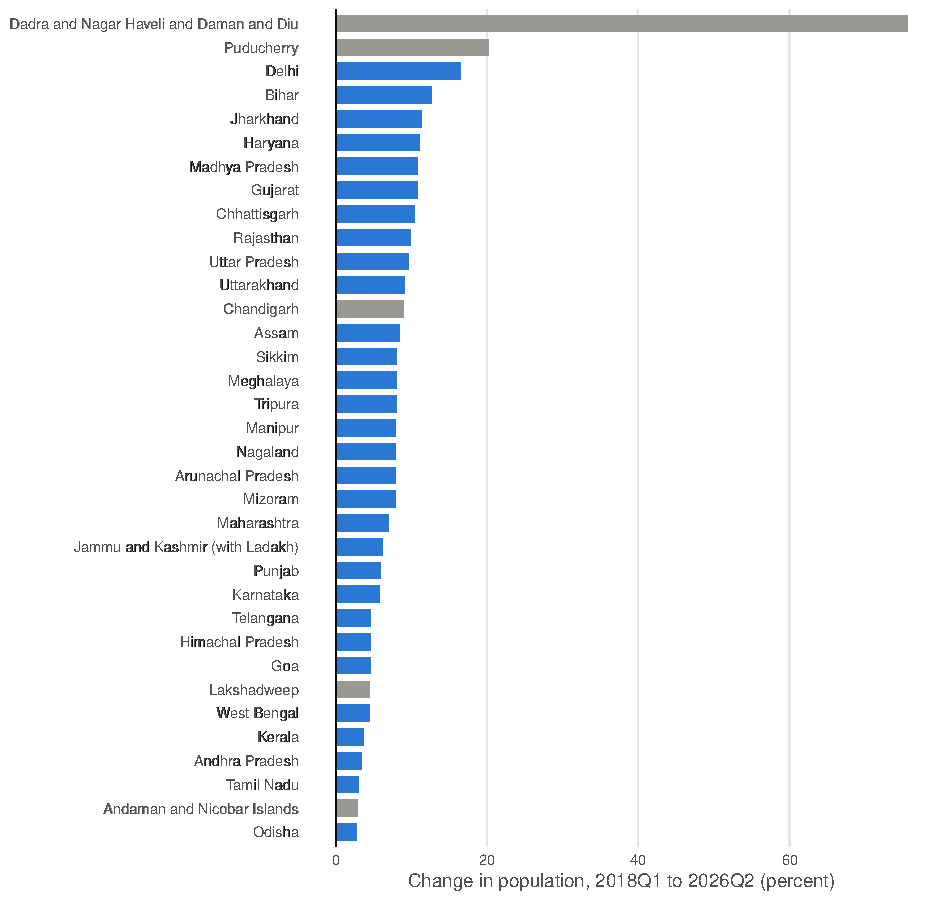
\includegraphics[width=\textwidth]{population_growth.pdf}
\caption{Population growth by state unit, 2018Q1 to 2026Q2. Unit: percent change. Sample: all \val{data.n_ids} state units; the other union territories are marked. Source: interpolation of the NCP 2020 projections \citep{ncp2020}.}\label{fig:population_growth}
\end{figure}

The figure sorts the state ids by growth, and grey bars mark the union territories outside the main sample. The largest growth is \val{pop.growth.max} percent, for \val{pop.growth.max.name}. The data of this study do not show the reason for this large value. A larger population gives smaller values per person, so the per-person values of this unit depend on this projection. In the main sample, the largest growth is \val{pop.growth.main.max} percent, for \val{pop.growth.main.max.name}. The smallest growth is \val{pop.growth.min} percent, for \val{pop.growth.min.name}. Bihar, Jharkhand and Haryana are near the top of the main sample, and Kerala, Andhra Pradesh and Tamil Nadu are near the bottom. In a state with fast population growth, a per-person value grows more slowly than its total. Thus these differences in growth matter for the comparison of states over time.

\subsection{Measures}\label{sec:measures}
For state $s$ and quarter $t$, let $C_{st}$ be the transaction count, $A_{st}$ the amount in nominal rupees, $U_{st}$ the registered users and $P_{st}$ the population. Let $C^k_{st}$ be the count of type $k$, where $k$ is P2P, Retail or Utility. The study uses these measures (without the subscripts):
\begin{align*}
\text{count per person} &= C/P, &
\text{amount per person} &= A/P, \\
\text{users per 1000 persons (reach)} &= 1000\,U/P, &
\text{transactions per user (intensity)} &= C/U, \\
\text{average transaction value} &= A/C, &
\text{type share} &= 100\,C^k/C.
\end{align*}

The count per person is the main measure of adoption. Its unit is transactions per person per quarter. It gives the number of PhonePe transactions in a quarter for each resident of the state. The amount per person is in rupees per person per quarter. It gives the value of these transactions for each resident. Reach is in registered users per 1000 persons. It shows how many registered users the app has for each 1000 persons in a state. It does not show how many of them used the app in the quarter. Intensity is in transactions per registered user per quarter. It shows how often a registered user pays with the app. The average transaction value is in rupees per transaction. The type share is the percent of the count of a state that is of type $k$. The P2P, Retail and Utility shares of a state add up to the whole count.

The growth of a variable $X$ from quarter $t-1$ to quarter $t$ is $100\,(X_t/X_{t-1} - 1)$ percent. The annual rate of growth from a first to a last quarter is $100\,[(X_1/X_0)^{1/n} - 1]$ percent. Here $X_0$ and $X_1$ are the values in the first and the last quarter, and $n$ is the number of years between them. The study gives growth rates from 2018Q4, not from 2018Q1. The national count is \val{nat.count.2018Q1} billion in 2018Q1 and \val{nat.count.2018Q4} billion in 2018Q4, so rates from 2018Q1 start from a much smaller base. Also, the national retail share moves between \val{nat.share.retail.min2018} and \val{nat.share.retail.max2018} percent during 2018.

Count per person is the product of reach and intensity: $C/P = (U/P)\,(C/U)$. Let $y = \ln(C/P)$, $r = \ln(U/P)$ and $i = \ln(C/U)$. Then $y = r + i$ for each state. Across the states of the main sample in one quarter, the variance of $y$ is thus $\operatorname{var}(y) = \operatorname{cov}(r, y) + \operatorname{cov}(i, y)$. Division by $\operatorname{var}(y)$ gives
\begin{equation}
1 = \frac{\operatorname{cov}(r, y)}{\operatorname{var}(y)} + \frac{\operatorname{cov}(i, y)}{\operatorname{var}(y)}.
\end{equation}
The first term is the contribution of reach, and the second term is the contribution of intensity. Each term is the slope of a least-squares line of $r$ (or $i$) on $y$ across the states. The reach term gives the part of the differences in adoption between states that goes with differences in reach. The intensity term gives the part that goes with differences in use per user. A term can be negative, and the other term is then larger than $1$. The decomposition shows how the differences divide between reach and intensity. It does not show a cause. Section~\ref{sec:states} gives the results for each quarter.

\section{Adoption in India as a whole}\label{sec:national}
This section describes the national series. The national value of a variable is the sum over the \val{data.n_ids} state ids. Section~\ref{sec:checks} shows that this sum equals the national files of PhonePe Pulse in each quarter. All amounts are nominal. Section~\ref{sec:totals} gives the totals and their growth (Figure~\ref{fig:national_totals} and Table~\ref{tab:annual}). Section~\ref{sec:qoq} gives the growth from quarter to quarter (Figure~\ref{fig:national_growth}). Section~\ref{sec:avg_value} gives the average transaction value (Figure~\ref{fig:avg_value}). Section~\ref{sec:types} gives the shares of the transaction types (Figure~\ref{fig:type_shares}).

\subsection{Totals and growth}\label{sec:totals}
Figure~\ref{fig:national_totals} shows the three national totals in each quarter: the transaction count, the amount and the registered users. Each panel has its own vertical scale, and each scale starts at zero.

\begin{figure}[tbp]
\centering
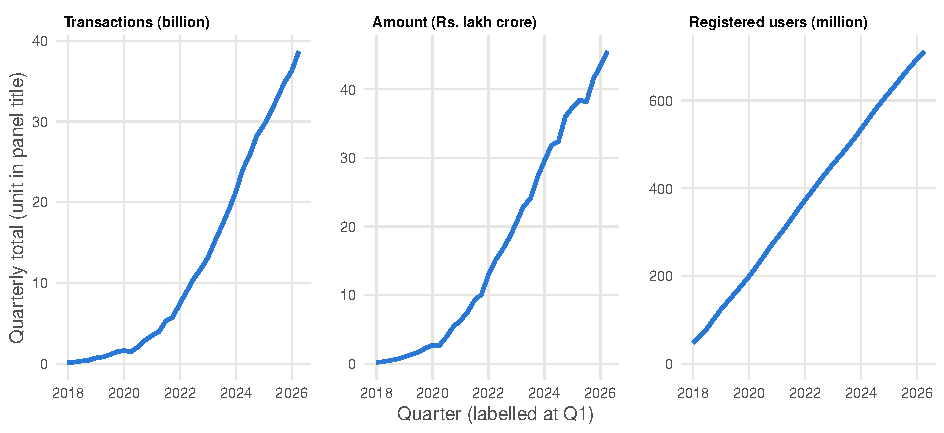
\includegraphics[width=\textwidth]{national_totals.pdf}
\caption{National transaction count (billion), transaction amount (Rs.\ lakh crore) and registered users (million), by quarter. Unit: national total of all \val{data.n_ids} state units. Period: 2018Q1--2026Q2. Source: \citet{phonepe_pulse}.}\label{fig:national_totals}
\end{figure}

The count increases from \val{nat.count.2018Q1} billion transactions in 2018Q1 to \val{nat.count.2026Q2} billion in 2026Q2. Thus the count of 2026Q2 is \val{nat.count_ratio} times the count of 2018Q1. The amount increases from Rs.~\val{nat.amount.2018Q1} lakh crore to Rs.~\val{nat.amount.2026Q2} lakh crore, a ratio of \val{nat.amount_ratio}. The registered users increase from \val{nat.users.2018Q1} million to \val{nat.users.2026Q2} million, a ratio of \val{nat.users_ratio}.

These ratios start from the small values of 2018Q1. Section~\ref{sec:measures} gives the reasons to measure growth from 2018Q4. From 2018Q4 to 2026Q2, the annual rate of growth is \val{nat.count_rate} percent for the count and \val{nat.amount_rate} percent for the amount. The annual rate for the registered users is \val{nat.users_rate} percent. The count grows faster than the amount, so the average value of a transaction decreases between the two quarters (Section~\ref{sec:avg_value}). The users grow more slowly than the count, so the number of transactions per user increases.

The shape of the user curve differs from the shapes of the other two curves. The user curve is almost a straight line. Each full year from \val{nat.users_added.first_year} to \val{nat.users_added.last_year} adds between \val{nat.users_added.min} and \val{nat.users_added.max} million registered users. An increase of almost the same size each year gives a rate of growth that decreases over time. The count and the amount curves rise slowly up to 2020 and more steeply after 2021.

Per person, the count increases from \val{nat.count_pc.2018Q1} transactions per person per quarter in 2018Q1 to \val{nat.count_pc.2018Q4} in 2018Q4. In 2026Q2, it is \val{nat.count_pc.2026Q2}. The registered users per 1000 persons increase from \val{nat.users_per_1000.2018Q1} in 2018Q1 to \val{nat.users_per_1000.2018Q4} in 2018Q4 and \val{nat.users_per_1000.2026Q2} in 2026Q2. This last value is not the share of persons who use PhonePe. The user count is a cumulative count of registrations, so it can include registrations that are no longer in use. The data also do not show whether one person can have more than one registration.

Table~\ref{tab:annual} gives the national values for each calendar year. The count and the amount are sums over the quarters of the year. The users are the value at the end of the year. The count per person is the annual count divided by the mean population of the quarters of the year. The year 2026 has only two quarters, so the table gives no growth rate for it.

\begin{table}[tbp]
\centering
\caption{National annual totals and growth. Unit: count in billion, amount in Rs.\ lakh crore (nominal), users at year end in million, count per person per year, average value in Rs., growth of count in percent. Sample: all \val{data.n_ids} state units. Period: calendar years 2018--2026 (2026 has two quarters). Source: \citet{phonepe_pulse}; population from \citet{ncp2020}.}\label{tab:annual}
\small
\begin{tabular}{@{}l r r r r r r@{}}
\toprule
 & Count & Amount & Users at & Count & Average & Growth \\
 & (billion) & (Rs.\ lakh & year end & per & value & of count \\
Year & & crore) & (million) & person & (Rs.) & (percent) \\
\midrule
2018 & 1.11 & 1.63 & 103.0 & 0.8 & 1{,}467 & -- \\
2019 & 4.12 & 6.29 & 179.9 & 3.1 & 1{,}525 & 271.9 \\
2020 & 8.02 & 14.65 & 266.2 & 5.9 & 1{,}827 & 94.5 \\
2021 & 18.45 & 33.09 & 351.7 & 13.5 & 1{,}793 & 130.0 \\
2022 & 38.64 & 62.97 & 436.0 & 28.0 & 1{,}630 & 109.4 \\
2023 & 64.30 & 94.60 & 513.0 & 46.2 & 1{,}471 & 66.4 \\
2024 & 99.33 & 129.71 & 598.7 & 70.8 & 1{,}306 & 54.5 \\
2025 & 128.54 & 155.38 & 676.8 & 90.8 & 1{,}209 & 29.4 \\
2026 (Q1--Q2) & 74.92 & 88.94 & 711.7 & 52.6 & 1{,}187 & -- \\
\bottomrule
\end{tabular}

\end{table}

The annual count increases in each year. Its rate of growth is \val{nat.ann.growth.2019} percent in 2019, \val{nat.ann.growth.2020} percent in 2020 and \val{nat.ann.growth.2021} percent in 2021. The rate of 2020 is thus lower than the rates of the years before and after it. The only fall of the national count, in 2020Q2, is in this year (Section~\ref{sec:qoq}). After 2021, the rate decreases in each year. It is \val{nat.ann.growth.2022} percent in 2022, \val{nat.ann.growth.2023} percent in 2023, \val{nat.ann.growth.2024} percent in 2024 and \val{nat.ann.growth.2025} percent in 2025.

The count per person increases from \val{nat.ann.count_pc.2018} transactions per person in 2018 to \val{nat.ann.count_pc.2025} in 2025. In 2025, the app records \val{nat.ann.count.2025} billion transactions with a total value of Rs.~\val{nat.ann.amount.2025} lakh crore. The annual average value is largest in \val{nat.ann.atv.max_year}, at Rs.~\val{nat.ann.atv.max}. It decreases in each later year, and it is Rs.~\val{nat.ann.atv.2025} in 2025.

\subsection{Quarter-on-quarter growth}\label{sec:qoq}
Figure~\ref{fig:national_growth} shows the change of the national count and of the national amount from the previous quarter, in percent. A bar below zero shows a quarter with a fall.

\begin{figure}[tbp]
\centering
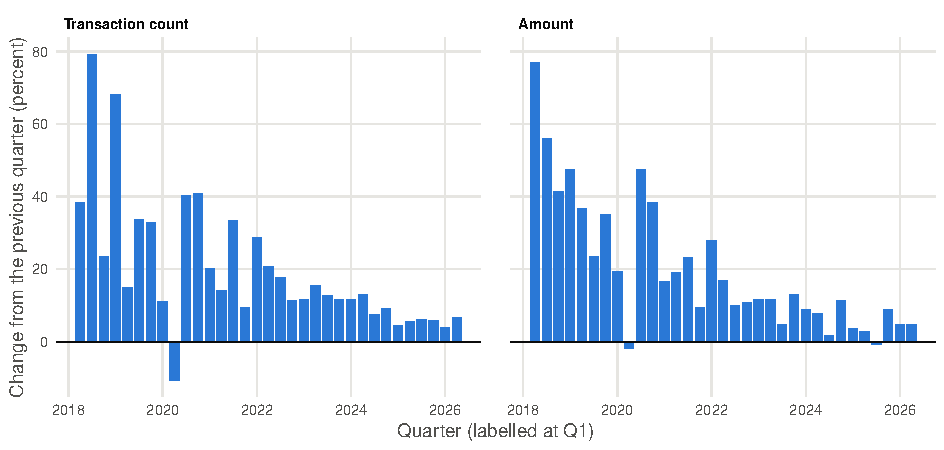
\includegraphics[width=\textwidth]{national_growth.pdf}
\caption{Quarter-on-quarter growth of the national transaction count and amount. Unit: percent change from the previous quarter. Sample: national total of all \val{data.n_ids} state units. Period: 2018Q2--2026Q2. Source: \citet{phonepe_pulse}.}\label{fig:national_growth}
\end{figure}

The growth of the count is largest in the first quarters, when the base is small. The largest value is \val{nat.qoq.count.max} percent, in \val{nat.qoq.count.max_period}. From 2018Q2 to 2024Q2, the median growth of the count is \val{nat.qoq.count.median_first} percent per quarter. In the last eight quarters, from 2024Q3 to 2026Q2, the median is \val{nat.qoq.count.median_last8} percent per quarter. Thus the count still grows in each recent quarter, but at a lower rate.

The only quarter with a fall in the national count is 2020Q2, the quarter from April to June 2020. The change of the count in this quarter is \val{nat.qoq.count.2020Q2} percent. The count goes from \val{nat.count.2020Q1} billion in 2020Q1 to \val{nat.count.2020Q2} billion in 2020Q2. The change of the amount is \val{nat.qoq.amount.2020Q2} percent, so the amount falls less than the count. The count falls in \val{nat.n_states_fall.2020Q2} of the \val{data.n_ids} state ids. In the other ids, the count of 2020Q2 is equal to or higher than the count of 2020Q1.

The fall does not continue. In 2020Q3, the count grows by \val{nat.qoq.count.2020Q3} percent to \val{nat.count.2020Q3} billion, which is more than the count of 2020Q1. The data of this study do not show the cause of the fall in 2020Q2.

The amount falls in the quarters \val{nat.qoq_neg_amount.periods}. The fall in the later quarter is small: the change is \val{nat.qoq.amount.neg_last} percent. The count does not fall in that quarter, so the average value of a transaction decreases.

\subsection{Average transaction value}\label{sec:avg_value}
The average transaction value is the amount divided by the count. Figure~\ref{fig:avg_value} shows it for India and for the states of the main sample. The national line is the national amount divided by the national count. The state line is the median of the \val{data.n_main} state values in each quarter. The band goes from the first to the third quartile of the state values.

\begin{figure}[tbp]
\centering
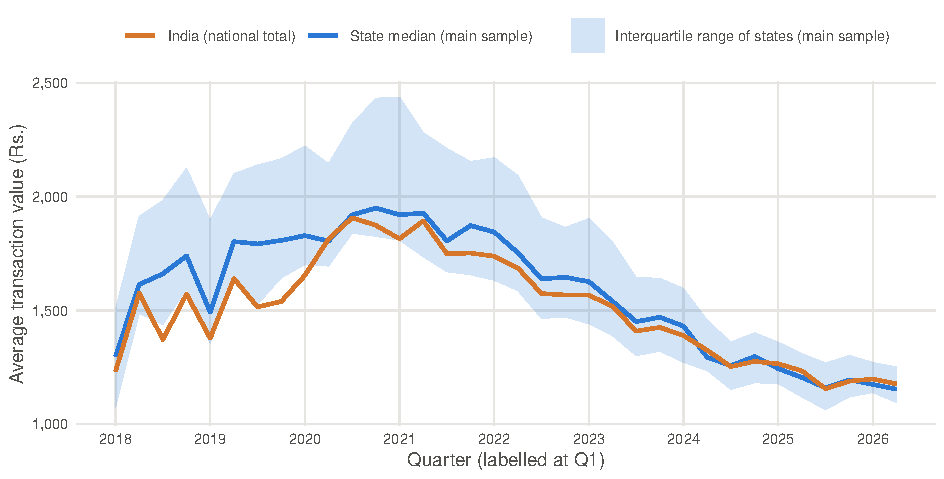
\includegraphics[width=\textwidth]{avg_value.pdf}
\caption{Average transaction value. Unit: Rs.\ per transaction (nominal), amount divided by count. Sample: national value, and median and interquartile range across the \val{data.n_main} main-sample states. Period: 2018Q1--2026Q2. Source: \citet{phonepe_pulse}.}\label{fig:avg_value}
\end{figure}

The national value is Rs.~\val{nat.atv.2018Q1} in 2018Q1. It rises, with large changes from quarter to quarter, to a peak of Rs.~\val{nat.atv.peak} in \val{nat.atv.peak_period}. After the peak, it is lower than in the previous quarter in \val{nat.atv.n_fall_after_peak} of \val{nat.atv.n_after_peak} quarters. In 2026Q2, it is Rs.~\val{nat.atv.2026Q2}, which is lower than the value of 2018Q1. In 2020Q2, the count falls more than the amount (Section~\ref{sec:qoq}), so the average value rises in that quarter.

The national value is a mean of the state values with the count of each state as its weight. The state median gives each state the same weight. The two lines thus differ, but they have a similar shape. The median has its largest value, Rs.~\val{st.atv.median.max}, in \val{st.atv.median.max_period}. In 2026Q2, the median is Rs.~\val{st.atv.median.2026Q2}.

The width of the band shows how much the states differ. The interquartile range is Rs.~\val{st.atv.iqr.2018Q4} in 2018Q4. It has its largest value, Rs.~\val{st.atv.iqr.max}, in \val{st.atv.iqr.max_period}. After that quarter, it decreases with some rises, and it is Rs.~\val{st.atv.iqr.2026Q2} in 2026Q2. Thus the average values of the states are closer to each other in 2026Q2 than in 2018Q4. In 2026Q2, the highest value in the main sample is Rs.~\val{st.atv.max}, in \val{st.atv.max.name}. The lowest is Rs.~\val{st.atv.min}, in \val{st.atv.min.name} (Table~\ref{tab:states}).

The fall of the average value and the rise of the retail share occur in the same years. From \val{nat.share.retail.min_period}, the retail share rises in most quarters (Section~\ref{sec:types}), and the average value falls. This pattern is consistent with a larger number of small payments to merchants. The study does not test this explanation. The type files give counts and no amounts, so the study cannot compute the average value of each type. The values are also nominal. Thus the study does not separate a change in prices from a change in the size of payments.

\subsection{Transaction types}\label{sec:types}
Figure~\ref{fig:type_shares} shows the national shares of the three types in the count: P2P, Retail and Utility. In each quarter, the three shares add up to the whole count.

\begin{figure}[tbp]
\centering
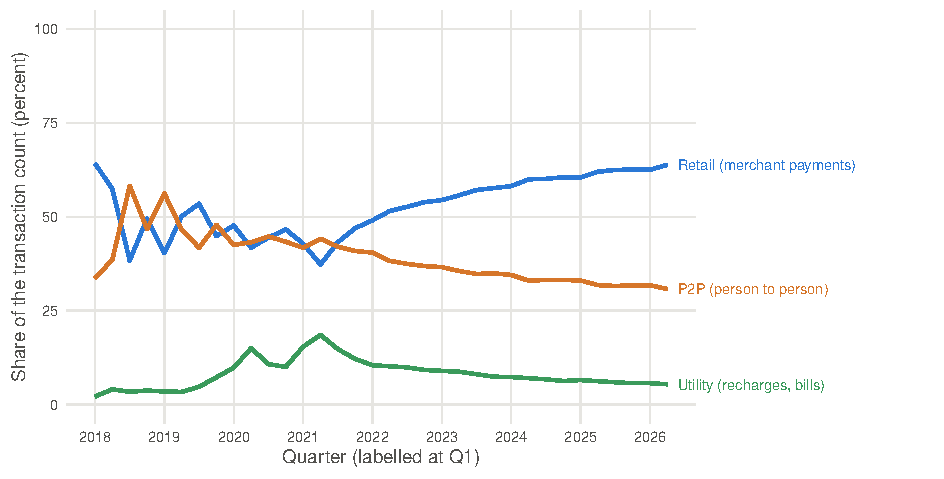
\includegraphics[width=\textwidth]{type_shares.pdf}
\caption{National shares of the transaction count by type: P2P, Retail and Utility. Unit: percent of the national count. Sample: national total of all \val{data.n_ids} state units. Period: 2018Q1--2026Q2. Source: \citet{phonepe_pulse}.}\label{fig:type_shares}
\end{figure}

The shares change by large amounts in 2018. In 2018Q1, the retail share is \val{nat.share.retail.2018Q1} percent and the P2P share is \val{nat.share.p2p.2018Q1} percent. During 2018, the retail share moves between \val{nat.share.retail.min2018} and \val{nat.share.retail.max2018} percent. In 2018Q4, the retail share is \val{nat.share.retail.2018Q4} percent, the P2P share is \val{nat.share.p2p.2018Q4} percent and the utility share is \val{nat.share.utility.2018Q4} percent. The data do not show the reason for these changes (Section~\ref{sec:limits}).

From 2019 to the middle of 2021, the retail and P2P shares are close to each other, and their order changes more than once. The utility share rises in the same years. It has its largest value, \val{nat.share.utility.max} percent, in \val{nat.share.utility.max_period}. In the same quarter, the retail share has its lowest value, \val{nat.share.retail.min} percent.

From \val{nat.share.retail_above_p2p_from}, the retail share is above the P2P share in every quarter. The retail share rises to \val{nat.share.retail.2026Q2} percent in 2026Q2, and the P2P share falls to \val{nat.share.p2p.2026Q2} percent. The utility share falls from its peak to \val{nat.share.utility.2026Q2} percent. Thus, in the recent quarters, payments to merchants are the largest type in the count. The retail share of 2026Q2 is close to that of 2018Q1, but the count is \val{nat.count_ratio} times larger.

The type shares are shares of the count, not of the amount. A payment to a merchant and a transfer to a person each count as one transaction. The data do not show which type has the larger payments. Thus the type shares do not show how the value of all payments divides between the types.

\section{Adoption across states}\label{sec:states}
This section compares the states. Statistics across states use the \val{data.n_main} states of the main sample. The figures and Table~\ref{tab:states} also show the \val{data.n_other_ut} other union territories. The reference quarters are 2018Q4 and 2026Q2. Section~\ref{sec:count_pc} compares the count per person (Figure~\ref{fig:state_count_pc} and Table~\ref{tab:states}). Section~\ref{sec:concentration} measures the concentration of activity in a few states (Table~\ref{tab:concentration}). Section~\ref{sec:persistence} measures how stable the order of the states is. Sections~\ref{sec:reach} and~\ref{sec:decomposition} divide the count per person into reach and intensity (Figures~\ref{fig:reach_intensity} and~\ref{fig:decomposition}, Table~\ref{tab:decomposition}). Section~\ref{sec:retail} compares the retail share with the count per person (Figure~\ref{fig:retail_share}).

\subsection{Transactions per person}\label{sec:count_pc}
Figure~\ref{fig:state_count_pc} shows the count per person of each state unit in 2018Q4 and in 2026Q2. The horizontal axis has a log scale, so equal distances show equal ratios. The open circle gives the value of 2018Q4, and the filled circle gives the value of 2026Q2. The units are in the order of their values in 2026Q2. Grey names mark the other union territories.

\begin{figure}[tbp]
\centering
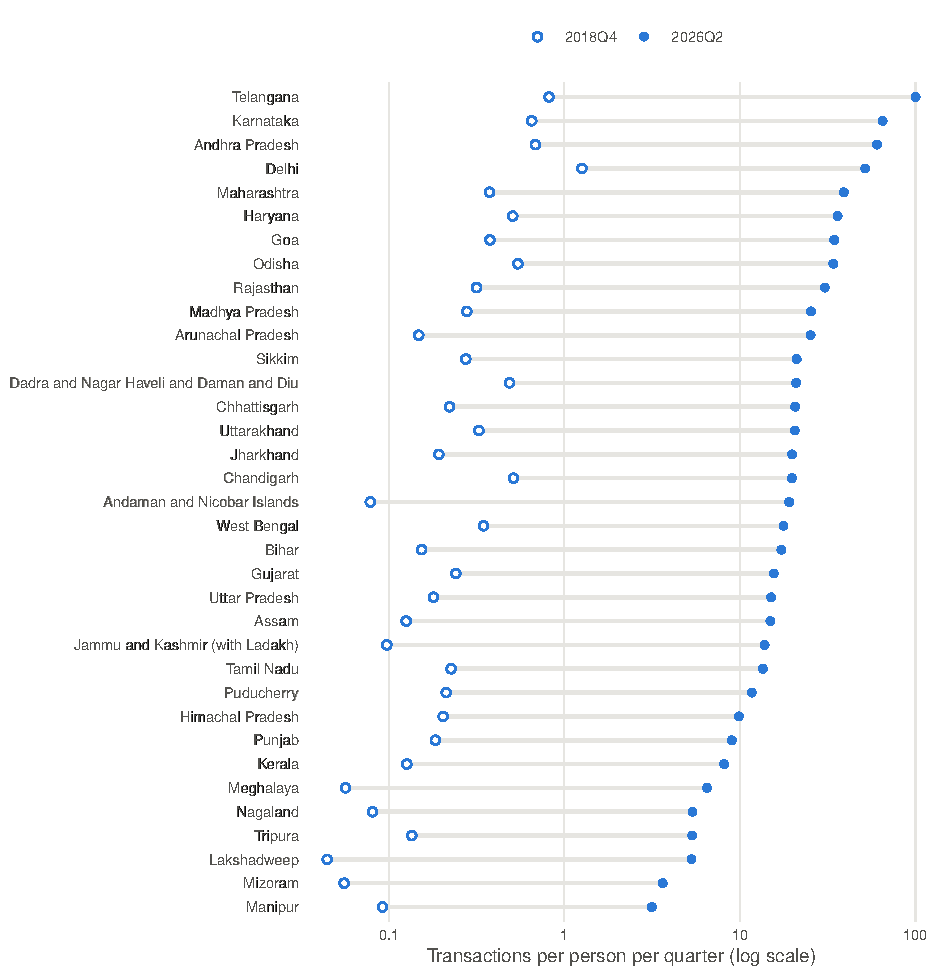
\includegraphics[width=\textwidth]{state_count_pc.pdf}
\caption{Transaction count per person per quarter, by state unit, in 2018Q4 and 2026Q2. Unit: transactions per person per quarter. Sample: all \val{data.n_ids} state units; the other union territories are marked. Source: \citet{phonepe_pulse}; population from \citet{ncp2020}.}\label{fig:state_count_pc}
\end{figure}

In 2018Q4, the count per person in the main sample goes from \val{st.count_pc.min.2018Q4} transactions per person per quarter, in \val{st.count_pc.min.name.2018Q4}, to \val{st.count_pc.max.2018Q4}, in \val{st.count_pc.max.name.2018Q4}. The ratio of the highest to the lowest value is \val{st.count_pc.maxmin.2018Q4}. This ratio uses the unrounded values, so it differs from the ratio of the two rounded values in the text. The median state has \val{st.count_pc.median.2018Q4} transactions per person per quarter. In this quarter, \val{st.n_above_nat.2018Q4} states have a value above the national value of \val{nat.count_pc.2018Q4}.

In 2026Q2, the lowest value is \val{st.count_pc.min.2026Q2}, in \val{st.count_pc.min.name.2026Q2}, and the highest value is \val{st.count_pc.max.2026Q2}, in \val{st.count_pc.max.name.2026Q2}. The ratio of the highest to the lowest value, also from unrounded values, is \val{st.count_pc.maxmin.2026Q2}. The median state has \val{st.count_pc.median.2026Q2} transactions per person per quarter. In this quarter, \val{st.n_above_nat.2026Q2} states are above the national value of \val{nat.count_pc.2026Q2}. The national value is a mean of the state values with population weights, so it is not the value of a typical state.

Every state of the main sample has a higher value in 2026Q2 than in 2018Q4. From 2018Q4 to 2026Q2, the annual rate of growth of the count per person goes from \val{st.count_pc_rate.min} percent, in \val{st.count_pc_rate.min.name}, to \val{st.count_pc_rate.max} percent, in \val{st.count_pc_rate.max.name}. Part 3 of the project tests whether the states with low values grow faster than the states with high values. This study does not test this relation.

Table~\ref{tab:states} gives the values of all state units in 2026Q2, in the order of the count per person. Next to the count per person, it gives the population, the amount per person, reach, intensity, the average value and the retail share. Thus the table shows the measures of Section~\ref{sec:measures} side by side for each unit.

\begin{table}[tbp]
\centering
\caption{State values in 2026Q2. Unit: population in million; count per person per quarter; amount per person in Rs.\ per quarter (nominal); users per 1000 persons; transactions per user per quarter; average value in Rs.; retail share in percent. Sample: all \val{data.n_ids} state units, sorted by count per person; $^\dagger$ marks the \val{data.n_other_ut} union territories outside the main sample. Source: \citet{phonepe_pulse}; population from \citet{ncp2020}.}\label{tab:states}
\small
\begin{tabular}{@{}>{\raggedright\arraybackslash}p{2.95cm} r r r r r r r@{}}
\toprule
 & Population & Count & Amount & Users & Count & Average & Retail \\
 & (million) & per & per person & per 1000 & per & value & share \\
Name & & person & (Rs.) & persons & user & (Rs.) & (percent) \\
\midrule
Telangana & 38.66 & 100.3 & 132{,}629 & 943 & 106.3 & 1{,}322 & 66.0 \\
Karnataka & 69.05 & 65.1 & 76{,}649 & 761 & 85.5 & 1{,}178 & 67.5 \\
Andhra Pradesh & 53.73 & 60.4 & 86{,}051 & 639 & 94.6 & 1{,}424 & 61.0 \\
Delhi & 22.64 & 51.8 & 51{,}967 & 939 & 55.1 & 1{,}004 & 68.5 \\
Maharashtra & 129.52 & 39.1 & 42{,}197 & 649 & 60.2 & 1{,}079 & 67.4 \\
Haryana & 31.38 & 36.0 & 40{,}263 & 728 & 49.5 & 1{,}117 & 67.9 \\
Goa & 1.60 & 34.5 & 43{,}161 & 842 & 41.0 & 1{,}251 & 67.9 \\
Odisha & 44.69 & 34.1 & 37{,}283 & 505 & 67.4 & 1{,}094 & 61.2 \\
Rajasthan & 83.82 & 30.5 & 38{,}052 & 521 & 58.4 & 1{,}249 & 64.2 \\
Madhya Pradesh & 89.89 & 25.4 & 28{,}572 & 446 & 57.0 & 1{,}125 & 63.8 \\
Arunachal Pradesh & 1.61 & 25.3 & 29{,}550 & 592 & 42.7 & 1{,}169 & 60.8 \\
Sikkim & 0.71 & 21.1 & 25{,}729 & 574 & 36.7 & 1{,}221 & 58.3 \\
Dadra and Nagar Haveli and Daman and Diu$^\dagger$ & 1.58 & 20.9 & 16{,}808 & 434 & 48.2 & 804 & 69.3 \\
Chhattisgarh & 31.29 & 20.7 & 21{,}684 & 422 & 49.0 & 1{,}050 & 62.3 \\
Uttarakhand & 12.02 & 20.6 & 21{,}235 & 562 & 36.6 & 1{,}033 & 66.4 \\
Jharkhand & 41.07 & 19.9 & 22{,}132 & 384 & 51.6 & 1{,}115 & 61.2 \\
Chandigarh$^\dagger$ & 1.27 & 19.8 & 19{,}877 & 653 & 30.3 & 1{,}004 & 71.0 \\
Andaman and Nicobar Islands$^\dagger$ & 0.41 & 19.1 & 25{,}704 & 543 & 35.1 & 1{,}347 & 63.4 \\
West Bengal & 100.60 & 17.7 & 21{,}986 & 430 & 41.2 & 1{,}241 & 56.4 \\
Bihar & 132.70 & 17.2 & 20{,}181 & 338 & 51.1 & 1{,}170 & 56.6 \\
Gujarat & 74.28 & 15.6 & 17{,}471 & 486 & 32.1 & 1{,}121 & 65.4 \\
Uttar Pradesh & 243.31 & 15.1 & 16{,}188 & 372 & 40.5 & 1{,}075 & 62.6 \\
Assam & 36.79 & 14.9 & 14{,}126 & 383 & 39.0 & 946 & 57.3 \\
Jammu and Kashmir (with Ladakh) & 14.22 & 13.8 & 15{,}360 & 415 & 33.4 & 1{,}109 & 62.3 \\
Tamil Nadu & 77.57 & 13.5 & 16{,}974 & 519 & 26.1 & 1{,}255 & 63.6 \\
Puducherry$^\dagger$ & 1.77 & 11.7 & 13{,}528 & 409 & 28.6 & 1{,}157 & 69.1 \\
Himachal Pradesh & 7.59 & 9.9 & 10{,}819 & 474 & 20.8 & 1{,}096 & 64.1 \\
Punjab & 31.36 & 9.0 & 11{,}788 & 450 & 20.0 & 1{,}309 & 62.7 \\
Kerala & 36.23 & 8.1 & 9{,}260 & 450 & 18.1 & 1{,}139 & 65.1 \\
Meghalaya & 3.45 & 6.5 & 7{,}059 & 238 & 27.3 & 1{,}086 & 48.4 \\
Nagaland & 2.30 & 5.4 & 7{,}123 & 262 & 20.5 & 1{,}325 & 49.2 \\
Tripura & 4.27 & 5.4 & 6{,}265 & 291 & 18.4 & 1{,}170 & 56.7 \\
Lakshadweep$^\dagger$ & 0.07 & 5.3 & 5{,}294 & 263 & 20.2 & 998 & 67.0 \\
Mizoram & 1.27 & 3.6 & 4{,}769 & 274 & 13.3 & 1{,}313 & 48.2 \\
Manipur & 3.32 & 3.2 & 5{,}118 & 257 & 12.2 & 1{,}623 & 43.5 \\
\bottomrule
\multicolumn{8}{@{}l}{\footnotesize $^\dagger$ Union territory outside the main sample.}\\
\end{tabular}

\end{table}

The five states with the highest count per person are \val{st.count_pc.top5.names.2026Q2}. The five states with the lowest values, from the lowest, are \val{st.count_pc.bottom5.names.2026Q2}. All five are in the north-east of India. Each of these five states has lower reach and lower intensity than each state of the top five.

The amount per person goes from Rs.~\val{st.amount_pc.min} per quarter in \val{st.amount_pc.min.name} to Rs.~\val{st.amount_pc.max} in \val{st.amount_pc.max.name}. The ratio of the two unrounded values is \val{st.amount_pc.maxmin}. The amount per person is the count per person times the average value. The average values of the states differ much less than their counts per person, so the two ratios are of similar size.

The size of a state does not decide its place in the table. The three states with the largest population are \val{st.pop.top3.names}. Of these states, \val{st.pop.top3.n_below_median} have a count per person below the median of the main sample. Thus a state with a large population can have a low count per person.

\subsection{Concentration}\label{sec:concentration}
Table~\ref{tab:concentration} shows how much of the national activity is in a few state units. For each reference quarter, it takes the five units with the largest transaction count. It gives their shares of the national count, amount, registered users and population. Its last row gives the smallest number of units that together have half of the national count. These statistics use all \val{data.n_ids} ids, because the national total is their sum.

\begin{table}[tbp]
\centering
\caption{Concentration of activity in the five states with the largest transaction count. Unit: share of the national total, in percent. Sample: all \val{data.n_ids} state units. Periods: 2018Q4 and 2026Q2. Source: \citet{phonepe_pulse}; population from \citet{ncp2020}.}\label{tab:concentration}
\small
\begin{tabular}{@{}l r r@{}}
\toprule
Share of the top five (by count) & 2018Q4 & 2026Q2 \\
\midrule
Transaction count (percent) & 46.2 & 52.6 \\
Amount (percent) & 44.1 & 53.7 \\
Registered users (percent) & 43.7 & 41.9 \\
Population (percent) & 42.2 & 37.5 \\
Units needed for half of all transactions & 6 & 5 \\
\bottomrule
\end{tabular}

\end{table}

In 2018Q4, the five units with the largest count are \val{conc.top5.names.2018Q4}. They have \val{conc.top5.count.2018Q4} percent of the count and \val{conc.top5.population.2018Q4} percent of the population. In 2026Q2, the five units are \val{conc.top5.names.2026Q2}. Their share of the count is \val{conc.top5.count.2026Q2} percent, and their share of the population is \val{conc.top5.population.2026Q2} percent. The set of five units changes between the two quarters, so the population share also changes. The share of the amount increases from \val{conc.top5.amount.2018Q4} to \val{conc.top5.amount.2026Q2} percent.

In both quarters, the five units have a larger share of the count than of the population. The difference is larger in 2026Q2. Their share of the registered users is \val{conc.top5.users.2018Q4} percent in 2018Q4 and \val{conc.top5.users.2026Q2} percent in 2026Q2. In 2026Q2, this share is closer to the population share than to the share of the count. Thus the registered users of these five units make more transactions per user than the users of the other units.

Half of the national count comes from \val{conc.n_half.2018Q4} units in 2018Q4 and from \val{conc.n_half.2026Q2} units in 2026Q2. Thus the count is more concentrated in the units with the largest counts at the end of the period than at the start.

\subsection{Rank persistence}\label{sec:persistence}
Figure~\ref{fig:state_count_pc} also shows that the order of the states changes little. The Spearman rank correlation of the count per person in 2018Q4 and in 2026Q2 is \val{st.rank_cor}. It uses the \val{data.n_main} states of the main sample, and average ranks for equal values. A value of $1$ means the same order in both quarters.

Of the \val{data.n_main} states, \val{st.n_rank_move_small} move by \val{st.rank_move.threshold} places or fewer between the two quarters. \val{st.rank_rise.name} moves up the most, from rank \val{st.rank_rise.r0} to rank \val{st.rank_rise.r1}. \val{st.rank_fall.names} move down the most, by \val{st.rank_fall.places} places each. \val{st.count_pc.max.name.2018Q4}, the highest state in 2018Q4, is still among the top five in 2026Q2.

This result agrees with \citet{reddy2024icrier}, who found little change in the ranks of states in an earlier release of the data. The two studies use different releases, so their numbers are not comparable (Section~\ref{sec:intro}). A stable order does not mean that the differences in level stay the same. Part 3 of the project measures how these differences change over time.

\subsection{Reach and intensity}\label{sec:reach}
Count per person is the product of reach and intensity (Section~\ref{sec:measures}). Figure~\ref{fig:reach_intensity} shows the two factors for each state unit in 2026Q2. The horizontal axis gives reach, in registered users per 1000 persons. The vertical axis gives intensity, in transactions per registered user per quarter. The labels are the two-letter codes of Appendix~\ref{app:units}, and grey labels mark the other union territories.

\begin{figure}[tbp]
\centering
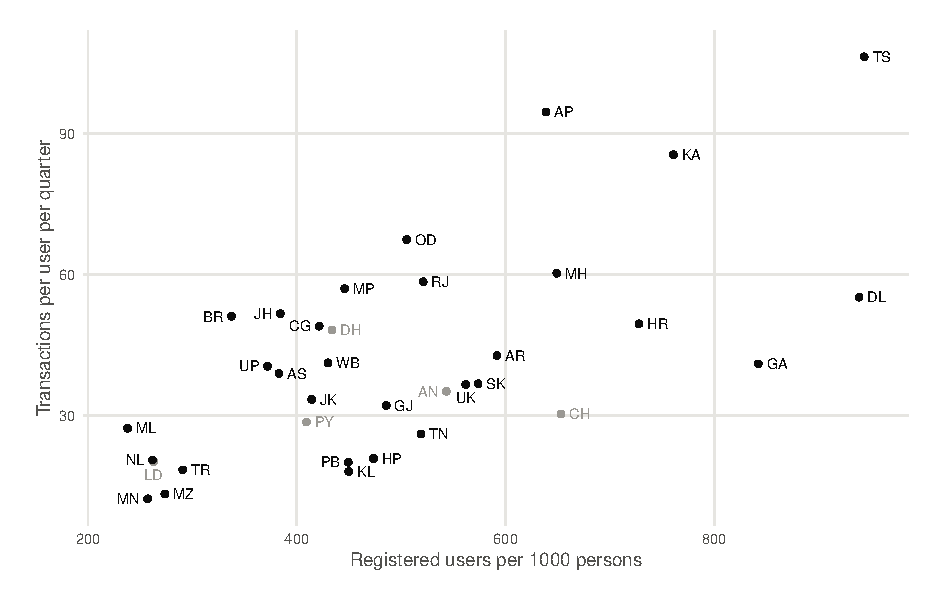
\includegraphics[width=\textwidth]{reach_intensity.pdf}
\caption{Reach against intensity in 2026Q2. Unit: registered users per 1000 persons (reach) and transactions per registered user per quarter (intensity). Sample: all \val{data.n_ids} state units; the other union territories are marked. Source: \citet{phonepe_pulse}; population from \citet{ncp2020}.}\label{fig:reach_intensity}
\end{figure}

Reach goes from \val{st.users_per_1000.min} registered users per 1000 persons in \val{st.users_per_1000.min.name} to \val{st.users_per_1000.max} in \val{st.users_per_1000.max.name}. Intensity goes from \val{st.intensity.min} transactions per user in \val{st.intensity.min.name} to \val{st.intensity.max} in \val{st.intensity.max.name}. With unrounded values, the ratio of the highest to the lowest value is \val{st.users_per_1000.maxmin} for reach and \val{st.intensity.maxmin} for intensity. Thus the states differ more in intensity than in reach. The north-eastern states with the lowest count per person are at the lower left of the figure, with low reach and low intensity.

The two factors go together, but not closely. Their Spearman rank correlation across the main sample is \val{st.reach_intensity_cor} in 2026Q2 and \val{st.reach_intensity_cor.2018Q4} in 2018Q4. Some states have a much higher rank in one factor than in the other. \val{st.ri_gap.reach.names} rank \val{st.ri_gap.reach.places} places higher in reach than in intensity. \val{st.ri_gap.intensity.names} ranks \val{st.ri_gap.intensity.places} places higher in intensity than in reach.

In the first group, reach is high, but each registered user makes few transactions. In the second group, reach is lower, but each registered user makes many transactions. A cumulative count of registrations can give the first pattern: registrations that are no longer in use increase reach and decrease intensity. The data cannot test this explanation, because they give no count of active users.

\subsection{Decomposition of the variance}\label{sec:decomposition}
Section~\ref{sec:measures} divides the cross-state variance of the log of the count per person into two parts. One part goes with reach, and the other part goes with intensity. Figure~\ref{fig:decomposition} shows the result for each quarter. The left panel shows the variances of $y$, $r$ and $i$ across the main sample. The right panel shows the two contributions, which add up to $1$ in each quarter. Table~\ref{tab:decomposition} gives the values for the two reference quarters.

\begin{figure}[tbp]
\centering
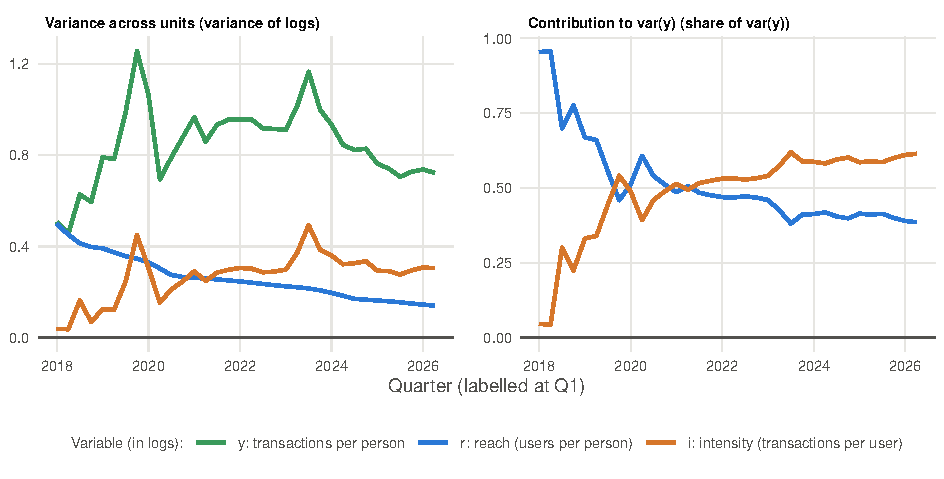
\includegraphics[width=\textwidth]{decomposition.pdf}
\caption{Contributions of reach and intensity to the cross-state variance of the log of transactions per person. Unit: share of the variance. Sample: the \val{data.n_main} main-sample states. Period: 2018Q1--2026Q2. Source: \citet{phonepe_pulse}; population from \citet{ncp2020}.}\label{fig:decomposition}
\end{figure}

\begin{table}[tbp]
\centering
\caption{Variance decomposition of the log of transactions per person: $y = \ln(C/P)$, reach $r = \ln(U/P)$ and intensity $i = \ln(C/U)$. Unit: variance of logs across states; contributions as shares of $\operatorname{var}(y)$. Sample: the \val{data.n_main} main-sample states. Periods: 2018Q4 and 2026Q2. Source: \citet{phonepe_pulse}; population from \citet{ncp2020}.}\label{tab:decomposition}
\small
\begin{tabular}{@{}l r r@{}}
\toprule
 & 2018Q4 & 2026Q2 \\
\midrule
$n$ & 30 & 30 \\
$\operatorname{var}(y)$ & 0.595 & 0.723 \\
$\operatorname{var}(r)$ & 0.397 & 0.140 \\
$\operatorname{var}(i)$ & 0.069 & 0.305 \\
$2\operatorname{cov}(r,i)$ & 0.129 & 0.278 \\
Reach contribution & 0.776 & 0.386 \\
Intensity contribution & 0.224 & 0.614 \\
\bottomrule
\end{tabular}

\end{table}

In 2018Q4, the contribution of reach is \val{dec.2018Q4.reach} and the contribution of intensity is \val{dec.2018Q4.intensity}. Thus most of the differences in adoption between states went with differences in reach. In 2026Q2, the contribution of reach is \val{dec.2026Q2.reach} and the contribution of intensity is \val{dec.2026Q2.intensity}. Now most of the differences go with differences in intensity.

The change occurs over several years. In 2018Q1, the contribution of reach is \val{dec.2018Q1.reach}. Intensity has the larger contribution for the first time in \val{dec.intensity_first_above}. From \val{dec.intensity_above_from}, it has the larger contribution in every quarter.

The variances in the left panel show how this change occurs. The variance of $r$ falls from \val{dec.2018Q4.var_r} in 2018Q4 to \val{dec.2026Q2.var_r} in 2026Q2. It decreases in every quarter of the period. The variance of $i$ increases from \val{dec.2018Q4.var_i} to \val{dec.2026Q2.var_i}. Thus the states become more similar in reach and less similar in intensity. The term $2\operatorname{cov}(r,i)$ in Table~\ref{tab:decomposition} also increases. This agrees with the higher rank correlation of reach and intensity in 2026Q2 (Section~\ref{sec:reach}).

The variance of $y$ does not move in one direction. It increases from \val{dec.2018Q4.var_y} in 2018Q4 to its largest value, \val{dec.var_y.max}, in \val{dec.var_y.max_period}. It then decreases and increases again to a second peak of \val{dec.var_y.max_late} in \val{dec.var_y.max_late_period}. In 2026Q2, it is \val{dec.2026Q2.var_y}. The variance of $i$ has its largest value, \val{dec.var_i.max}, in \val{dec.var_i.max_period}. Thus the second peak of $\operatorname{var}(y)$ goes with a large spread in intensity.

The decomposition describes how the differences between states divide between reach and intensity. It does not show a cause. Part 3 of the project uses the change of the differences over time in its test of convergence. This study gives only the values.

\subsection{Retail share}\label{sec:retail}
Figure~\ref{fig:retail_share} shows the retail share of each state unit against its count per person in 2026Q2. The horizontal axis has a log scale. Grey labels mark the other union territories.

\begin{figure}[tbp]
\centering
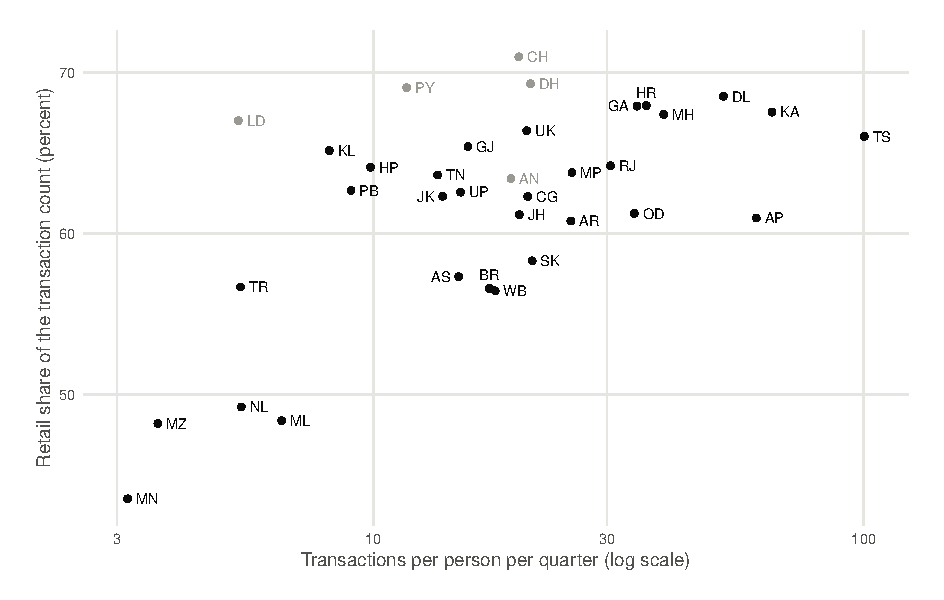
\includegraphics[width=\textwidth]{retail_share.pdf}
\caption{Retail share of the transaction count against transactions per person in 2026Q2. Unit: percent of the state count; transactions per person per quarter. Sample: all \val{data.n_ids} state units; the other union territories are marked. Source: \citet{phonepe_pulse}; population from \citet{ncp2020}.}\label{fig:retail_share}
\end{figure}

In the main sample, the retail share goes from \val{retail.min} percent in \val{retail.min.name} to \val{retail.max} percent in \val{retail.max.name}. \val{retail.min.name} also has the lowest count per person. The Spearman rank correlation of the retail share and the count per person is \val{retail.cor.2026Q2}. Thus the states with more transactions per person tend to have a larger share of payments to merchants. Of the other union territories, \val{retail.n_other_above} have a retail share above the highest value of the main sample. They are outside the main sample, so they do not enter the correlation.

In 2018Q4, the same coefficient is \val{retail.cor.2018Q4}, with the opposite sign. The type shares of 2018 change by large amounts from quarter to quarter (Section~\ref{sec:types}). Thus the study does not interpret the coefficient of 2018Q4.

The correlation of 2026Q2 does not show a cause. More payments to merchants can increase adoption, or high adoption can bring more merchants to the app. The data of this study cannot separate these two directions.

\section{Limitations of the data}\label{sec:limits}
The panel measures the use of one app. PhonePe Pulse covers the transactions of PhonePe, not all UPI transactions. The share of PhonePe in UPI can differ between states. If it does, the panel shows differences between states that are not differences in UPI use. The share can also change over time. Then the growth rates of this study differ from the growth of UPI. This study does not measure the share of PhonePe. Part 2 compares the PhonePe values with the NPCI state data for the quarters from April 2025.

The user count is a count of registrations, not of active users or of persons. The count does not fall in any of the \val{check.users_fall.n} pairs of consecutive quarters (Section~\ref{sec:checks}). This result is consistent with a cumulative count, which keeps the users who no longer use the app. Thus reach can increase in a state while the use of the app does not. The data do not show whether one person can have more than one registration. They also do not show whether a registration moves to a new state when a user moves. Thus reach is not the share of persons who use the app.

The repository does not document how PhonePe assigns a transaction or a user to a state. The README gives the hover count as the transactions done in the quarter for the state. It gives the top user lists as the states that users registered from. It does not say whether the state comes from the address of the user, the location of the device or the location of the merchant. Thus the panel cannot show where a payment between two states goes. A state with many persons who live or work in another state can have values that do not match its resident population.

The population values are projections, not counts. NCP 2020 makes them from the 2011 Census and the Sample Registration System (Section~\ref{sec:data}). The study has no population count for any quarter of the panel. An error in a projection goes directly into each per-person value of that state, and the size of the errors is not known. The per-person values of \val{pop.growth.max.name}, with the largest projected growth, depend most on the projection (Section~\ref{sec:population}). For Goa and most union territories, the report uses a mathematical method that does not project fertility, mortality and migration.

All amounts are nominal. The amount per person and the average value thus include the change in prices over the period. A change in the average value can come from a change in prices or from a change in the size of payments. This study cannot separate the two. The count is a number of transactions, not a value. Thus the growth of the count and the count per person need no price adjustment. Part 2 converts the amounts to real values with the consumer price indices \citep{mospi_cpi}.

The type shares change by large amounts in 2018. The national retail share moves between \val{nat.share.retail.min2018} and \val{nat.share.retail.max2018} percent in that year. The data do not show whether these changes come from changes in use or from the restated definitions of the types (Section~\ref{sec:pulse}). For this reason, the study uses 2018Q4 and not 2018Q1 as the first reference quarter, and it does not interpret the type shares of 2018. The type files also give counts only, so the study cannot divide the amount by type.

\section{Conclusions}\label{sec:conclusions}
This part builds a state-quarter panel of PhonePe adoption for \val{data.n_ids} state units and \val{data.n_quarters} quarters, from 2018Q1 to 2026Q2. The denominator is the quarterly population from the NCP 2020 projections. All data checks pass. The type counts sum to the state counts, and the state files sum to the national files in each quarter. The panel gives the findings below. All values are nominal.

First, the national count grows at an annual rate of \val{nat.count_rate} percent from 2018Q4 to 2026Q2. It reaches \val{nat.count.2026Q2} billion transactions in 2026Q2, or \val{nat.count_pc.2026Q2} transactions per person per quarter. The growth becomes lower over time. The median growth per quarter is \val{nat.qoq.count.median_first} percent up to 2024Q2 and \val{nat.qoq.count.median_last8} percent in the last eight quarters. The count falls only in 2020Q2, with a change of \val{nat.qoq.count.2020Q2} percent.

Second, the average transaction value has a peak of Rs.~\val{nat.atv.peak} in \val{nat.atv.peak_period} and falls to Rs.~\val{nat.atv.2026Q2} in 2026Q2. In the same years, the retail share of the count increases from \val{nat.share.retail.min} percent in \val{nat.share.retail.min_period} to \val{nat.share.retail.2026Q2} percent. This pattern is consistent with more small payments to merchants. The data do not give the amount by type, so the study does not test this explanation.

Third, the differences in adoption between states are large, and the order of the states is stable. The ratio of the highest to the lowest count per person in the main sample is \val{st.count_pc.maxmin.2018Q4} in 2018Q4 and \val{st.count_pc.maxmin.2026Q2} in 2026Q2. The Spearman rank correlation of the state values in the two quarters is \val{st.rank_cor}.

Fourth, the activity is concentrated in a few states. In 2026Q2, the five units with the largest count have \val{conc.top5.count.2026Q2} percent of the count and \val{conc.top5.population.2026Q2} percent of the population. Half of the national count comes from \val{conc.n_half.2026Q2} units.

Fifth, the source of the differences between states changes from reach to intensity. The contribution of reach to the cross-state variance of the log count per person is \val{dec.2018Q4.reach} in 2018Q4 and \val{dec.2026Q2.reach} in 2026Q2. The contribution of intensity increases from \val{dec.2018Q4.intensity} to \val{dec.2026Q2.intensity}.

Sixth, the states with more transactions per person have larger retail shares. In 2026Q2, the Spearman rank correlation of the retail share and the count per person is \val{retail.cor.2026Q2}. The data do not show the direction of this relation.

The later parts of the project use this panel. Part 2 converts the amounts to real values with state consumer price indices. It also compares the PhonePe values with the NPCI state data to measure the share of PhonePe in UPI. It shows the measures on maps. Part 3 uses the count per person of the main sample to test convergence. It tests whether the states with low adoption move closer to the leading states. The results of this part are descriptive. They do not answer the questions of Parts 2 and 3.

\bibliographystyle{plainnat}
\bibliography{../../references/refs}

\appendix
\section{The state units}\label{app:units}
The names in the last two columns are the raw names after the normalisation of the state crosswalk: lower case, with ``and'' in place of ``\&''. A semicolon separates the raw names that the crosswalk sums into one unit.

\small
\begin{longtable}{@{}>{\raggedright\arraybackslash}p{2.8cm} l l l >{\raggedright\arraybackslash}p{2.8cm} >{\raggedright\arraybackslash}p{2.8cm}@{}}
\caption{The 35 state units of the panel: display name, \texttt{state\_id}, two-letter code \citep{iso3166_2_in}, membership of the main sample of 30, and the raw names that map to the unit in the PhonePe Pulse hover file for 2026Q2 \citep{phonepe_pulse} and in NCP 2020, Table 8 \citep{ncp2020}. Source: state crosswalk (\texttt{state\_crosswalk.csv}) and state labels (\texttt{state\_labels.csv}).}\label{tab:units}\\
\toprule
Name & \texttt{state\_id} & Code & Main & PhonePe raw names & NCP raw names \\
\midrule
\endfirsthead
\toprule
Name & \texttt{state\_id} & Code & Main & PhonePe raw names & NCP raw names \\
\midrule
\endhead
Andaman and Nicobar Islands & \texttt{andaman\_nicobar} & AN & No & andaman and nicobar islands & andaman and nicobar islands \\
Andhra Pradesh & \texttt{andhra\_pradesh} & AP & Yes & andhra pradesh & andhra pradesh \\
Arunachal Pradesh & \texttt{arunachal\_pradesh} & AR & Yes & arunachal pradesh & arunachal pradesh \\
Assam & \texttt{assam} & AS & Yes & assam & assam \\
Bihar & \texttt{bihar} & BR & Yes & bihar & bihar \\
Chandigarh & \texttt{chandigarh} & CH & No & chandigarh & chandigarh \\
Chhattisgarh & \texttt{chhattisgarh} & CG & Yes & chhattisgarh & chhattisgarh \\
Dadra and Nagar Haveli and Daman and Diu & \texttt{dnh\_dd} & DH & No & dadra and nagar haveli and daman and diu & dadra and nagar haveli; daman and diu \\
Delhi & \texttt{delhi} & DL & Yes & delhi & nct of delhi \\
Goa & \texttt{goa} & GA & Yes & goa & goa \\
Gujarat & \texttt{gujarat} & GJ & Yes & gujarat & gujarat \\
Haryana & \texttt{haryana} & HR & Yes & haryana & haryana \\
Himachal Pradesh & \texttt{himachal\_pradesh} & HP & Yes & himachal pradesh & himachal pradesh \\
Jammu and Kashmir (with Ladakh) & \texttt{jammu\_kashmir} & JK & Yes & jammu and kashmir; ladakh & jammu and kashmir; ladakh \\
Jharkhand & \texttt{jharkhand} & JH & Yes & jharkhand & jharkhand \\
Karnataka & \texttt{karnataka} & KA & Yes & karnataka & karnataka \\
Kerala & \texttt{kerala} & KL & Yes & kerala & kerala \\
Lakshadweep & \texttt{lakshadweep} & LD & No & lakshadweep & lakshadweep \\
Madhya Pradesh & \texttt{madhya\_pradesh} & MP & Yes & madhya pradesh & madhya pradesh \\
Maharashtra & \texttt{maharashtra} & MH & Yes & maharashtra & maharashtra \\
Manipur & \texttt{manipur} & MN & Yes & manipur & manipur \\
Meghalaya & \texttt{meghalaya} & ML & Yes & meghalaya & meghalaya \\
Mizoram & \texttt{mizoram} & MZ & Yes & mizoram & mizoram \\
Nagaland & \texttt{nagaland} & NL & Yes & nagaland & nagaland \\
Odisha & \texttt{odisha} & OD & Yes & odisha & odisha \\
Puducherry & \texttt{puducherry} & PY & No & puducherry & puducherry \\
Punjab & \texttt{punjab} & PB & Yes & punjab & punjab \\
Rajasthan & \texttt{rajasthan} & RJ & Yes & rajasthan & rajasthan \\
Sikkim & \texttt{sikkim} & SK & Yes & sikkim & sikkim \\
Tamil Nadu & \texttt{tamil\_nadu} & TN & Yes & tamil nadu & tamil nadu \\
Telangana & \texttt{telangana} & TS & Yes & telangana & telangana \\
Tripura & \texttt{tripura} & TR & Yes & tripura & tripura \\
Uttar Pradesh & \texttt{uttar\_pradesh} & UP & Yes & uttar pradesh & uttar pradesh \\
Uttarakhand & \texttt{uttarakhand} & UK & Yes & uttarakhand & uttarakhand \\
West Bengal & \texttt{west\_bengal} & WB & Yes & west bengal & west bengal \\
\bottomrule
\end{longtable}

\normalsize

\section{Reproduction}\label{app:repro}
The commands below run from the repository root. They fetch the raw files, build the interim files, write the figures, tables and numbers, and build this document.
\begin{verbatim}
make data analysis report
\end{verbatim}
The PhonePe Pulse files are at the commit \texttt{257bf38e3095020f9f516c4c72c10bdc348781b1}. The study reads these input files:
\begin{itemize}
\item \path{data/interim/phonepe.csv}
\item \path{data/interim/phonepe_types.csv}
\item \path{data/interim/phonepe_checks.csv}
\item \path{data/interim/population.csv}
\item \path{src/R/lib/state_labels.csv}
\end{itemize}
The script \path{src/R/part1_study.R} writes the figures to \path{output/study/part1/figures/}, the tables to \path{output/study/part1/tables/} and the numbers to \path{output/study/part1/numbers.tex}. The file \path{numbers.tex} is generated. Do not edit it. A number in the text comes from this file with the command \verb|\val|, and an unknown key stops the compile.

\end{document}
